% Preview of the Experiment 2 thesis assets. Preamble: the packages of the thesis's
% dissertation.tex that tables and figures use (uathesis print layout: A4, 12 pt, scale 0.75,
% 5 mm binding offset). algorithm.sty is omitted (not installed on this machine; unused here).
\documentclass[a4paper,12pt,openany]{book}
\usepackage[a4paper,hmarginratio=1:1,vmarginratio=1:1,scale=0.75,bindingoffset=5mm]{geometry}
\usepackage{graphicx}
\usepackage{cmap}
\usepackage{amssymb}
\usepackage{amsmath}
\usepackage{setspace}
\usepackage{booktabs}
\usepackage{url}
\usepackage{adjustbox}
\usepackage{tabularx}
\usepackage{tabularray}
\usepackage{multicol}
\usepackage{subcaption}
\usepackage[inline]{enumitem}
\usepackage[table,usenames,dvipsnames]{xcolor}
\usepackage[figuresright]{rotating}  % thesis: figuresright keeps multi-page sideways floats facing one way
\usepackage{makecell}
\usepackage[unicode=true,colorlinks=true,linkcolor=black]{hyperref}
\usepackage{cleveref}
% thesis-tablestyle.tex -- one table style for the whole thesis (every chapter, generated or hand-written).
%
% Load ONCE in the preamble, after xcolor (with its `table' option) and booktabs:
%     \usepackage[table,usenames,dvipsnames]{xcolor}   % already in dissertation.tex
%     \usepackage{booktabs}                            % already in dissertation.tex
%     \input{thesis-tablestyle}
%
% What it does, in every table / table* / sidewaystable / sidewaystable* float:
%   * zebra striping of the body rows (header rows stay white), in a very light grey that prints in greyscale;
%   * slightly taller rows (\arraystretch times \thesisrowstretch, on top of any \arraystretch the table sets);
%   * booktabs rules keep their spacing; where a rule follows a shaded row, the gap above the rule is shaded
%     too, so there is no white band.
% The body starts after the first \midrule (booktabs) or the second \hline (\hline tables). Striping restarts
% after every \midrule, so a group row after a \midrule (e.g. "\multicolumn{8}{l}{\textit{PropNEAT}}") is
% white and its rows alternate below it. A table whose header ends without a \midrule says how many header
% rows it has: \thesistablestyle[1]. A table with no top rule (\toprule or \hline) is not striped.
%
% Switches (in the preamble for the whole thesis, or inside one table for that table):
%   \thesisstripestrue / \thesisstripesfalse        zebra on (default) / off
%   \thesisfiverulestrue / \thesisfiverulesfalse    thin grey rule every \thesisfiveevery body rows (default off);
%                                                   the alternative to stripes: \thesisstripesfalse\thesisfiverulestrue
%   \thesistablesautotrue / \thesistablesautofalse  apply to every table float automatically (default on); when
%                                                   off, only tables that call \thesistablestyle are styled
%   \renewcommand\thesisrowstretch{1.1}             row-height factor (1 = unchanged)
%   \renewcommand\thesisfiveevery{5}                rows between the thin rules
%   \definecolor{thesisstripe}{gray}{0.93}          stripe colour (and thesisfiverule for the thin rules)
% Per table:
%   \thesistablestyle[<n>]   apply the style (generated tables call it first; idempotent); <n> = number of
%                            header rows after \toprule when the header does not end with a \midrule
%   \thesisnostripes         opt out: this table keeps its own look (no stripes, no thin rules, no extra
%                            height). Use it for tables that colour their own cells or rows, or use \multirow
%                            (the next row's shading would cover the \multirow text).
% Nested tabulars (\makecell, a tabular inside a cell) are left alone and do not disturb the outer striping.
\makeatletter
\@ifpackageloaded{colortbl}{}{\RequirePackage{colortbl}}
\@ifpackageloaded{booktabs}{}{\RequirePackage{booktabs}}
\@ifundefined{fpeval}{\RequirePackage{xfp}}{}

\newif\ifthesisstripes   \thesisstripestrue
\newif\ifthesisfiverules \thesisfiverulesfalse
\newif\ifthesistablesauto \thesistablesautotrue
\definecolor{thesisstripe}{gray}{0.93}
\definecolor{thesisfiverule}{gray}{0.6}
\newcommand\thesisrowstretch{1.1}
\newcommand\thesisfiveevery{5}

\newif\ifthesis@active   % inside a styled float
\newif\ifthesis@engine   % stripes or thin rules are being drawn
\newif\ifthesis@data     % past the header
\newif\ifthesis@firstrule
\newif\ifthesis@lastrow  % the last item was a row (not a rule)
\newif\ifthesis@curgrey  % the current row is shaded
\newif\ifthesis@lastgrey % the row just ended was shaded
\newif\ifthesis@wantsep
\newif\ifthesis@oksep
\newcount\thesis@row     % body row number since the last \midrule (1 = first)
\newcount\thesis@five
\newcount\thesis@head    % header rows still to come (-1: wait for a \midrule)
\newcount\thesis@lvl     % group level of the outer table's \noalign (-1: unknown)
\thesis@lvl=\m@ne
\def\thesis@headrows{-1}

% ---- row colours (colortbl's per-row colour, as xcolor's \rowcolors sets it). colortbl extends each
% cell's colour by \tabcolsep on both sides; at an @{} edge that would stick out past the rules, so the
% first / last cell of a row drops that overhang when the column spec starts / ends with @{}.
\newif\ifthesis@leftflush
\newif\ifthesis@rightflush
\newcount\thesis@cellno
\newcount\thesis@ncols
% colortbl stretches a cell's colour with 1fill against the cell's own 1fill of alignment glue; a
% \makecell adds its own \hfill glue (counted in \thesis@mc), which would take part of the stretch and
% leave the right of the cell white. The colour's stretch is raised to match (\thesis@k).
\newcount\thesis@mc
\def\thesis@k{1}
\def\thesis@mcell#1#2\@nil#3{\thesis@o@mcell{#1}#2\@nil{#3}%
  \ifx\mcell@left\hfill\global\advance\thesis@mc\@ne\fi
  \ifx\mcell@right\hfill\global\advance\thesis@mc\@ne\fi}
\def\thesis@docolor{\global\let\CT@do@color\relax
  \@tempdima\wd\z@\advance\@tempdima\@tempdimb\advance\@tempdima\@tempdimc
  \kern-\@tempdimb\leaders\vrule\hskip\@tempdima\@plus\thesis@k fill
  \kern-\@tempdimc\hskip-\wd\z@\@plus-\thesis@k fill\relax}
\def\thesis@cellstep{%
  \def\thesis@k{1}%
  \ifnum\currentgrouplevel=\thesis@lvl
    \edef\thesis@k{\the\numexpr\@ne+\thesis@mc\relax}\global\thesis@mc\z@
    \global\advance\thesis@cellno\@ne
    % overlap the next cell a little, so screen renderers show no hairline gaps between cells
    \ifnum\thesis@cellno<\thesis@ncols\advance\@tempdimc.25pt\fi
    \ifnum\thesis@cellno=\@ne\ifthesis@leftflush\@tempdimb\z@\fi\fi
    \ifnum\thesis@cellno=\thesis@ncols\ifthesis@rightflush\@tempdimc\z@\fi\fi
  \fi}
\def\thesis@grey{\gdef\CT@row@color{\thesis@cellstep\CT@color{thesisstripe}}\global\thesis@curgreytrue}
\def\thesis@white{\gdef\CT@row@color{\thesis@cellstep}\global\thesis@curgreyfalse}
\ExplSyntaxOn
\cs_new_protected:Npn \thesis@edges #1
  {
    \str_set:Nn \l_tmpa_str {#1}
    \str_remove_all:Nn \l_tmpa_str { ~ }
    \str_if_eq:eeTF { \str_head:N \l_tmpa_str } { @ }
      { \global\thesis@leftflushtrue } { \global\thesis@leftflushfalse }
    \str_if_eq:eeTF { \str_range:Nnn \l_tmpa_str { -3 } { -1 } } { \tl_to_str:n { @{} } }
      { \global\thesis@rightflushtrue } { \global\thesis@rightflushfalse }
  }
\ExplSyntaxOff
\def\thesis@array[#1]#2{%
  \ifnum\thesis@lvl<\z@\thesis@edges{#2}\else\ifnum\currentgrouplevel<\thesis@lvl\thesis@edges{#2}\fi\fi
  \thesis@o@array[#1]{#2}}
\def\thesis@colour{\ifthesisstripes\ifodd\thesis@row\thesis@white\else\thesis@grey\fi\else\thesis@white\fi}
\def\thesis@startdata{\global\thesis@datatrue\global\thesis@head\m@ne\global\thesis@row\@ne
  \global\thesis@five\z@\thesis@colour}
\def\thesis@sethead{\global\thesis@lvl\currentgrouplevel\global\thesis@firstrulefalse
  \global\thesis@ncols\z@\global\thesis@cellno\z@
  \global\thesis@datafalse\global\thesis@row\z@\global\thesis@five\z@\thesis@white
  \global\thesis@head=\thesis@headrows\relax\ifnum\thesis@head=\z@\thesis@startdata\fi}

% ---- at every row end (\CT@everycr); only the outer table's rows count
\def\thesis@close{\ifnum0=`{\fi}}
\def\thesis@cr{\noalign{\ifnum0=`}\fi\thesis@crstep}
\def\thesis@crstep{\thesis@wantsepfalse
  \ifnum\currentgrouplevel=\thesis@lvl
    \ifthesis@curgrey\global\thesis@lastgreytrue\else\global\thesis@lastgreyfalse\fi
    \global\thesis@lastrowtrue
    \ifnum\thesis@cellno>\thesis@ncols\global\thesis@ncols\thesis@cellno\fi
    \global\thesis@cellno\z@\global\thesis@mc\z@
    \ifthesis@data
      \global\advance\thesis@row\@ne\thesis@colour
      \ifthesisfiverules
        \global\advance\thesis@five\@ne
        \ifnum\thesis@five<\thesisfiveevery\relax\else\global\thesis@five\z@\thesis@wantseptrue\fi
      \fi
    \else
      \thesis@white
      \ifnum\thesis@head>\z@
        \global\advance\thesis@head\m@ne
        \ifnum\thesis@head=\z@\thesis@startdata\fi
      \fi
    \fi
  \fi
  \ifthesis@wantsep\expandafter\thesis@peek\else\expandafter\thesis@close\fi}
% a thin rule after every \thesisfiveevery body rows, unless a rule or the end comes next
\def\thesis@peek{\futurenonspacelet\thesis@next\thesis@decide}
\def\thesis@nosepif#1{\ifx\thesis@next#1\thesis@oksepfalse\fi}
\def\thesis@decide{\thesis@okseptrue
  \thesis@nosepif\bottomrule\thesis@nosepif\midrule\thesis@nosepif\toprule\thesis@nosepif\cmidrule
  \thesis@nosepif\hline\thesis@nosepif\cline\thesis@nosepif\addlinespace\thesis@nosepif\specialrule
  \thesis@nosepif\end\thesis@nosepif\noalign\thesis@nosepif\crcr
  \ifthesis@oksep{\color{thesisfiverule}\hrule\@height\cmidrulewidth}\fi
  \thesis@close}

% ---- rules: #1 = 0 \cmidrule, 1 \toprule, 2 \midrule, 3 \bottomrule, 4 \hline
\def\thesis@fill{{\color{thesisstripe}\hrule\@height\aboverulesep}\vskip-\aboverulesep}
\def\thesis@rule#1{\noalign{\thesis@rulestep#1}}
\def\thesis@rulestep#1{%
  \ifnum#1=\@ne\thesis@sethead\else
  \ifnum#1=4
    \ifthesis@firstrule\thesis@sethead\else
    \ifnum\currentgrouplevel=\thesis@lvl\thesis@startdata\else\thesis@sethead\fi\fi
  \else
  \ifnum\currentgrouplevel=\thesis@lvl
    \ifthesis@lastrow\ifthesis@lastgrey\thesis@fill\fi\fi
    \ifnum#1=\tw@\thesis@startdata\fi
    \ifnum#1=\thr@@\global\thesis@datafalse\thesis@white\fi
  \fi\fi\fi
  \global\thesis@lastrowfalse}

% ---- at the start of each tabular / tabularx / tabular* (not nested ones): reset, taller rows
\def\thesis@tabbegin{%
  \ifthesis@active
    \ifnum\thesis@lvl<\z@\thesis@tabreset\else
    \ifnum\currentgrouplevel<\thesis@lvl\thesis@tabreset\fi\fi
  \fi}
\def\thesis@tabreset{\global\thesis@lvl\m@ne\global\thesis@firstruletrue\global\thesis@datafalse
  \global\thesis@row\z@\global\thesis@five\z@\global\thesis@head\m@ne\global\thesis@lastrowfalse
  \global\thesis@curgreyfalse
  \edef\arraystretch{\fpeval{\arraystretch*\thesisrowstretch}}}
\AddToHook{env/tabular/begin}{\thesis@tabbegin}
\AddToHook{env/tabular*/begin}{\thesis@tabbegin}
\AddToHook{env/tabularx/begin}{\thesis@tabbegin}

% ---- the style itself
\newcommand\thesistablestyle[1][-1]{%
  \def\thesis@headrows{#1}%
  \ifthesis@active\else
    \thesis@activetrue\global\thesis@lvl\m@ne
    \thesis@enginefalse
    \ifthesisstripes\thesis@enginetrue\fi
    \ifthesisfiverules\thesis@enginetrue\fi
    \ifthesis@engine
      \CT@everycr{\the\everycr\thesis@cr}%
      \let\thesis@o@toprule\toprule\def\toprule{\thesis@rule1\thesis@o@toprule}%
      \let\thesis@o@midrule\midrule\def\midrule{\thesis@rule2\thesis@o@midrule}%
      \let\thesis@o@bottomrule\bottomrule\def\bottomrule{\thesis@rule3\thesis@o@bottomrule}%
      \let\thesis@o@cmidrule\cmidrule\def\cmidrule{\thesis@rule0\thesis@o@cmidrule}%
      \let\thesis@o@hline\hline\def\hline{\thesis@rule4\thesis@o@hline}%
      \ifdefined\@@array\let\thesis@o@array\@@array\let\@@array\thesis@array\fi
      \ifdefined\mcell@@@tabular\let\thesis@o@mcell\mcell@@@tabular\let\mcell@@@tabular\thesis@mcell\fi
      \let\thesis@o@docolor\CT@@do@color\let\CT@@do@color\thesis@docolor
    \fi
  \fi}
\newcommand\thesisnostripes{%
  \ifthesis@active
    \thesis@activefalse
    \ifthesis@engine
      \CT@everycr{\noalign{\global\let\CT@row@color\relax}\the\everycr}%
      \let\toprule\thesis@o@toprule\let\midrule\thesis@o@midrule\let\bottomrule\thesis@o@bottomrule
      \let\cmidrule\thesis@o@cmidrule\let\hline\thesis@o@hline
      \ifdefined\thesis@o@array\let\@@array\thesis@o@array\fi
      \ifdefined\thesis@o@mcell\let\mcell@@@tabular\thesis@o@mcell\fi
      \let\CT@@do@color\thesis@o@docolor
      \thesis@enginefalse
    \fi
  \fi}
\def\thesis@auto{\ifthesistablesauto\thesistablestyle\fi}
\AddToHook{env/table/begin}{\thesis@auto}
\AddToHook{env/table*/begin}{\thesis@auto}
\AddToHook{env/sidewaystable/begin}{\thesis@auto}
\AddToHook{env/sidewaystable*/begin}{\thesis@auto}
\makeatother
  % thesis table style (loaded once in the thesis preamble)
\newcolumntype{Y}{>{\centering\arraybackslash}X}
\renewcommand\floatpagefraction{.9}
\renewcommand\topfraction{.9}
\renewcommand\bottomfraction{.9}
\renewcommand\textfraction{.1}
\setcounter{totalnumber}{50}
\setcounter{topnumber}{50}
\setcounter{bottomnumber}{50}
\graphicspath{{../figures/}}   % the figure floats use the Overleaf paths figures/ch7/<id>.pdf (flat)
\begin{document}
\chapter*{Experiment 2: tables and figures (preview)}
Generated by \texttt{thesis/ch7/exp2/make\_assets.py}. References:
Tables~\ref{tab:exp2-headline}--\ref{tab:exp2-s8-families}, Figures~\ref{fig:exp2-auc}--\ref{fig:exp2-heart-pairs}.

\section*{Every run, per dataset}
% Generated by thesis/ch7/exp2/per_run.py (via make_assets.py) -- do not edit by hand.
\begin{sidewaystable}
  \centering
  \footnotesize
  \setlength{\tabcolsep}{2.5pt}
  \renewcommand{\arraystretch}{1.15}
  \begin{adjustbox}{max width=\textheight}
  \begin{tabular}{@{}rccccccccccccccc@{}}
    \toprule
    Seed & \makecell{Train\\AUC} & \makecell{Test AUC\\(95\% CI)} & \makecell{Inputs\\used} & \makecell{Hidden\\nodes} & \makecell{Enabled\\conn.} & \makecell{Skippiness\\(skip conn.)} & Density & Depth & \makecell{Leaf $+$\\comp.} & Splits & \makecell{Id.\\nodes} & \makecell{Coverage\\struct./comp.} & \makecell{Function\\pres.\ error} & \makecell{Agent\\min} & \makecell{Mike\\min} \\
    \midrule
    s0 & 0.906 & 0.903 {\scriptsize [0.896, 0.909]} & 51/107 & 11 & 70 & 1.38 (11) & 0.138 & 3 & 10 $+$ 1 & 6 & 1 & 1.00/1.00 & $5.6\times10^{-16}$ & 19.3 & 6 \\
    s1 & 0.907 & 0.904 {\scriptsize [0.898, 0.911]} & 50/107 & 16 & 80 & 3.81 (14) & 0.143 & 7 & 7 $+$ 1 & 7 & 6 & 1.00/1.00 & $4.4\times10^{-16}$ & 28.2 & 4 \\
    s2 & 0.906 & 0.903 {\scriptsize [0.897, 0.910]} & 60/107 & 16 & 91 & 1.06 (9) & 0.148 & 3 & 8 $+$ 1 & 9 & 1 & 1.00/1.00 & $6.7\times10^{-16}$ & 21.3 & 8 \\
    s3 & \textbf{0.913} & \textbf{0.909} {\scriptsize [0.902, 0.915]} & 63/107 & 15 & 85 & 1.63 (14) & 0.151 & 4 & 12 $+$ 1 & 5 & 1 & 1.00/1.00 & $5.6\times10^{-16}$ & 21.1 & -- \\
    s4 & 0.910 & 0.907 {\scriptsize [0.901, 0.914]} & 55/107 & 15 & 81 & 2.63 (13) & 0.125 & 5 & 12 $+$ 3 & 0 & 12 & 1.00/1.00 & $4.4\times10^{-16}$ & 24.2 & 5 \\
    s5 & 0.912 & 0.907 {\scriptsize [0.901, 0.914]} & 66/107 & 15 & 95 & 1.64 (17) & 0.154 & 4 & 8 $+$ 2 & 9 & 1 & 1.00/1.00 & $7.8\times10^{-16}$ & 21.7 & 2 \\
    s6 & 0.908 & 0.905 {\scriptsize [0.899, 0.911]} & 53/107 & 15 & 77 & 1.82 (14) & 0.131 & 4 & 8 $+$ 1 & 5 & 1 & 1.00/1.00 & $5.0\times10^{-16}$ & 21.4 & 2 \\
    s7 & 0.910 & 0.908 {\scriptsize [0.901, 0.914]} & 65/107 & 15 & 95 & 1.87 (18) & 0.130 & 4 & 11 $+$ 2 & 12 & 1 & 1.00/1.00 & $6.1\times10^{-16}$ & 28.8 & 4 \\
    s8 & 0.911 & \textbf{0.909} {\scriptsize [0.903, 0.915]} & 63/107 & 15 & 89 & 2.40 (15) & 0.146 & 5 & 6 $+$ 2 & 8 & 1 & 1.00/1.00 & $7.2\times10^{-16}$ & 25.4 & 2 \\
    s9 & 0.907 & 0.906 {\scriptsize [0.899, 0.912]} & 61/107 & 17 & 91 & 2.32 (16) & 0.127 & 5 & 7 $+$ 1 & 7 & 1 & 1.00/1.00 & $6.7\times10^{-16}$ & 21.0 & 4 \\
    \midrule
    \makecell[l]{Median\\(range)} & \makecell{0.909\\{\scriptsize 0.906--0.913}} & \makecell{0.906\\{\scriptsize 0.903--0.909}} & \makecell{60.5\\{\scriptsize 50--66}} & \makecell{15\\{\scriptsize 11--17}} & \makecell{87\\{\scriptsize 70--95}} & \makecell{1.84\\{\scriptsize 1.06--3.81}} & \makecell{0.140\\{\scriptsize 0.125--0.154}} & \makecell{4\\{\scriptsize 3--7}} & \makecell{9.5\\{\scriptsize 8--15}} & \makecell{7\\{\scriptsize 0--12}} & \makecell{1\\{\scriptsize 1--12}} & 10/10 full & $\le$ $7.8\times10^{-16}$ & \makecell{21.5\\{\scriptsize 19.3--28.8}} & \makecell{4\\{\scriptsize 2--8}} \\
    \bottomrule
  \end{tabular}
  \end{adjustbox}
  \caption{Adult (income; 10 seeds $\times$ 100 generations, pre-registered): every run. AUCs are of the best genome of the run; the test interval is a percentile bootstrap (10{,}000 resamples). \emph{Inputs used}: inputs with an enabled path to the output, of the 107 model inputs (one-hot columns counted separately). \emph{Hidden nodes}, \emph{enabled connections}, \emph{depth} (edges on the longest input-to-output path; layers $=$ depth $+\,1$) and \emph{skip connections} (edges that jump a layer, direct input-to-output edges excluded) are of the phenotype. \emph{Skippiness} (mean number of layers a connection gene skips) and \emph{density} (node and connection genes over the parameters of a dense network with the same layer widths) are the library's \texttt{ExplaNEAT} measures on the genome. Explanation: leaf $+$ composition annotations, node splits and identity nodes of the frozen-method (v4) explanation; structural / compositional coverage; \emph{function-preservation error}, the largest absolute difference between the explained model and the network on the training rows. \emph{Agent min}: the explaining agent's wall-clock minutes; \emph{Mike min}: the author's verification minutes. Seed s3 has no verification minutes in its record; the median is over the other 9.}
  \label{tab:exp2-runs-adult}
\end{sidewaystable}

% Generated by thesis/ch7/exp2/per_run.py (via make_assets.py) -- do not edit by hand.
\begin{sidewaystable}
  \centering
  \footnotesize
  \setlength{\tabcolsep}{2.5pt}
  \renewcommand{\arraystretch}{1.15}
  \begin{adjustbox}{max width=\textheight}
  \begin{tabular}{@{}rccccccccccccccc@{}}
    \toprule
    Seed & \makecell{Train\\AUC} & \makecell{Test AUC\\(95\% CI)} & \makecell{Inputs\\used} & \makecell{Hidden\\nodes} & \makecell{Enabled\\conn.} & \makecell{Skippiness\\(skip conn.)} & Density & Depth & \makecell{Leaf $+$\\comp.} & Splits & \makecell{Id.\\nodes} & \makecell{Coverage\\struct./comp.} & \makecell{Function\\pres.\ error} & \makecell{Agent\\min} & \makecell{Mike\\min} \\
    \midrule
    s0 & 0.908 & 0.895 {\scriptsize [0.860, 0.927]} & 45/71 & 23 & 89 & 1.43 (25) & 0.133 & 4 & 8 $+$ 1 & 12 & 1 & 1.00/1.00 & $5.6\times10^{-16}$ & 16.2 & 8 \\
    s1 & 0.910 & \textbf{0.904} {\scriptsize [0.870, 0.934]} & 38/71 & 27 & 92 & 3.46 (31) & 0.141 & 9 & 6 $+$ 1 & 13 & 1 & 1.00/1.00 & $3.3\times10^{-16}$ & 16.6 & 6 \\
    s2 & 0.901 & 0.876 {\scriptsize [0.839, 0.909]} & 49/71 & 20 & 94 & 2.59 (29) & 0.141 & 6 & 6 $+$ 3 & 18 & 1 & 1.00/1.00 & $7.8\times10^{-16}$ & 23.3 & 3 \\
    s3 & 0.899 & 0.888 {\scriptsize [0.855, 0.919]} & 47/71 & 16 & 77 & 1.54 (15) & 0.168 & 4 & 12 $+$ 3 & 7 & 2 & 1.00/1.00 & $4.4\times10^{-16}$ & 24.4 & 1 \\
    s4 & 0.898 & 0.883 {\scriptsize [0.849, 0.914]} & 40/71 & 13 & 64 & 1.09 (12) & 0.154 & 3 & 8 $+$ 3 & 12 & 2 & 1.00/1.00 & $4.4\times10^{-16}$ & 20.4 & 7 \\
    s5 & 0.901 & 0.881 {\scriptsize [0.845, 0.914]} & 44/71 & 16 & 75 & 1.73 (19) & 0.204 & 5 & 5 $+$ 1 & 2 & 5 & 1.00/1.00 & $4.4\times10^{-16}$ & 18.9 & 4 \\
    s6 & 0.910 & 0.895 {\scriptsize [0.860, 0.927]} & 46/71 & 18 & 84 & 2.41 (21) & 0.171 & 6 & 7 $+$ 2 & 7 & 4 & 1.00/1.00 & $5.6\times10^{-16}$ & 19.9 & 5 \\
    s7 & \textbf{0.919} & 0.900 {\scriptsize [0.866, 0.932]} & 36/71 & 14 & 59 & 2.59 (15) & 0.181 & 6 & 7 $+$ 2 & 5 & 2 & 1.00/1.00 & $1.0\times10^{-15}$ & 15.7 & 3 \\
    s8 & 0.905 & 0.873 {\scriptsize [0.836, 0.908]} & 47/71 & 16 & 79 & 2.17 (17) & 0.220 & 6 & 6 $+$ 4 & 9 & 2 & 1.00/1.00 & $7.2\times10^{-16}$ & 17.4 & 1 \\
    s9 & 0.892 & 0.875 {\scriptsize [0.840, 0.907]} & 46/71 & 21 & 85 & 2.78 (24) & 0.171 & 7 & 8 $+$ 1 & 8 & 1 & 1.00/1.00 & $4.4\times10^{-16}$ & 16.5 & 2 \\
    \midrule
    \makecell[l]{Median\\(range)} & \makecell{0.903\\{\scriptsize 0.892--0.919}} & \makecell{0.886\\{\scriptsize 0.873--0.904}} & \makecell{45.5\\{\scriptsize 36--49}} & \makecell{17\\{\scriptsize 13--27}} & \makecell{81.5\\{\scriptsize 59--94}} & \makecell{2.29\\{\scriptsize 1.09--3.46}} & \makecell{0.169\\{\scriptsize 0.133--0.220}} & \makecell{6\\{\scriptsize 3--9}} & \makecell{9\\{\scriptsize 6--15}} & \makecell{8.5\\{\scriptsize 2--18}} & \makecell{2\\{\scriptsize 1--5}} & 10/10 full & $\le$ $1.0\times10^{-15}$ & \makecell{18.1\\{\scriptsize 15.7--24.4}} & \makecell{4\\{\scriptsize 1--8}} \\
    \bottomrule
  \end{tabular}
  \end{adjustbox}
  \caption{Churn (10 seeds $\times$ 100 generations): every run. AUCs are of the best genome of the run; the test interval is a percentile bootstrap (10{,}000 resamples). \emph{Inputs used}: inputs with an enabled path to the output, of the 71 model inputs (one-hot columns counted separately). \emph{Hidden nodes}, \emph{enabled connections}, \emph{depth} (edges on the longest input-to-output path; layers $=$ depth $+\,1$) and \emph{skip connections} (edges that jump a layer, direct input-to-output edges excluded) are of the phenotype. \emph{Skippiness} (mean number of layers a connection gene skips) and \emph{density} (node and connection genes over the parameters of a dense network with the same layer widths) are the library's \texttt{ExplaNEAT} measures on the genome. Explanation: leaf $+$ composition annotations, node splits and identity nodes of the frozen-method (v4) explanation; structural / compositional coverage; \emph{function-preservation error}, the largest absolute difference between the explained model and the network on the training rows. \emph{Agent min}: the explaining agent's wall-clock minutes; \emph{Mike min}: the author's verification minutes.}
  \label{tab:exp2-runs-churn}
\end{sidewaystable}

% Generated by thesis/ch7/exp2/per_run.py (via make_assets.py) -- do not edit by hand.
\begin{sidewaystable}
  \centering
  \footnotesize
  \setlength{\tabcolsep}{2.5pt}
  \renewcommand{\arraystretch}{1.15}
  \begin{adjustbox}{max width=\textheight}
  \begin{tabular}{@{}rccccccccccccccc@{}}
    \toprule
    Seed & \makecell{Train\\AUC} & \makecell{Test AUC\\(95\% CI)} & \makecell{Inputs\\used} & \makecell{Hidden\\nodes} & \makecell{Enabled\\conn.} & \makecell{Skippiness\\(skip conn.)} & Density & Depth & \makecell{Leaf $+$\\comp.} & Splits & \makecell{Id.\\nodes} & \makecell{Coverage\\struct./comp.} & \makecell{Function\\pres.\ error} & \makecell{Agent\\min} & \makecell{Mike\\min} \\
    \midrule
    s0 & 0.953 & 0.899 {\scriptsize [0.810, 0.968]} & 22/26 & 10 & 43 & 2.97 (12) & 0.268 & 7 & 4 $+$ 3 & 7 & 1 & 1.00/1.00 & $2.2\times10^{-16}$ & 11.9 & 7 \\
    s1 & 0.951 & 0.895 {\scriptsize [0.809, 0.961]} & 17/26 & 8 & 33 & 1.62 (8) & 0.416 & 5 & 4 $+$ 1 & 4 & 1 & 1.00/1.00 & $3.3\times10^{-16}$ & 11.4 & 4 \\
    s2 & 0.959 & \textbf{0.926} {\scriptsize [0.853, 0.978]} & 17/26 & 13 & 50 & 2.44 (24) & 0.230 & 6 & 5 $+$ 3 & 13 & 1 & 1.00/1.00 & $4.4\times10^{-16}$ & 13.5 & 10 \\
    s3 & 0.952 & 0.899 {\scriptsize [0.811, 0.965]} & 20/26 & 10 & 45 & 2.12 (12) & 0.238 & 5 & 7 $+$ 2 & 10 & 2 & 1.00/1.00 & $3.3\times10^{-16}$ & 15.3 & 7 \\
    s4 & 0.954 & 0.889 {\scriptsize [0.796, 0.962]} & 20/26 & 8 & 37 & 2.27 (12) & 0.246 & 5 & 5 $+$ 2 & 6 & 1 & 1.00/1.00 & $3.3\times10^{-16}$ & 14.1 & 3 \\
    s5 & 0.953 & 0.913 {\scriptsize [0.833, 0.972]} & 23/26 & 7 & 40 & 1.87 (6) & 0.480 & 5 & 4 $+$ 3 & 5 & 1 & 1.00/1.00 & $3.3\times10^{-16}$ & 12.9 & 3 \\
    s6 & 0.958 & 0.863 {\scriptsize [0.760, 0.946]} & 18/26 & 6 & 34 & 2.12 (13) & 0.297 & 5 & 4 $+$ 4 & 9 & 1 & 1.00/1.00 & $4.4\times10^{-16}$ & 13.8 & 5 \\
    s7 & 0.959 & 0.889 {\scriptsize [0.798, 0.959]} & 22/26 & 11 & 48 & 2.03 (15) & 0.254 & 5 & 6 $+$ 2 & 9 & 3 & 1.00/1.00 & $3.3\times10^{-16}$ & 12.5 & 6 \\
    s8 & \textbf{0.964} & 0.883 {\scriptsize [0.787, 0.959]} & 19/26 & 9 & 40 & 1.47 (11) & 0.524 & 5 & 4 $+$ 2 & 6 & 2 & 1.00/1.00 & $2.2\times10^{-16}$ & 12.4 & 8 \\
    s9 & 0.960 & 0.874 {\scriptsize [0.777, 0.949]} & 22/26 & 5 & 35 & 0.76 (6) & 0.503 & 3 & 4 $+$ 1 & 7 & 1 & 1.00/1.00 & $3.3\times10^{-16}$ & 13.3 & 4 \\
    \midrule
    \makecell[l]{Median\\(range)} & \makecell{0.956\\{\scriptsize 0.951--0.964}} & \makecell{0.892\\{\scriptsize 0.863--0.926}} & \makecell{20\\{\scriptsize 17--23}} & \makecell{8.5\\{\scriptsize 5--13}} & \makecell{40\\{\scriptsize 33--50}} & \makecell{2.08\\{\scriptsize 0.76--2.97}} & \makecell{0.283\\{\scriptsize 0.230--0.524}} & \makecell{5\\{\scriptsize 3--7}} & \makecell{7\\{\scriptsize 5--9}} & \makecell{7\\{\scriptsize 4--13}} & \makecell{1\\{\scriptsize 1--3}} & 10/10 full & $\le$ $4.4\times10^{-16}$ & \makecell{13.1\\{\scriptsize 11.4--15.3}} & \makecell{6\\{\scriptsize 3--10}} \\
    \bottomrule
  \end{tabular}
  \end{adjustbox}
  \caption{Heart-100: every run. Bold: the column's best AUC.}
  \label{tab:exp2-runs-heart100}
\end{sidewaystable}

\clearpage
\section*{Signals, per dataset}
% Generated by thesis/ch7/exp2/signal_tables.py (via make_assets.py) -- do not edit by hand.
\begin{sidewaystable}
  \centering
  \footnotesize
  \setlength{\tabcolsep}{2.6pt}
  \begin{tabularx}{\textheight}{@{}>{\raggedright\arraybackslash}X*{10}{c}>{\raggedright\arraybackslash}p{4.4cm}@{}}
    \toprule
    Signal & s0 & s1 & s2 & s3 & s4 & s5 & s6 & s7 & s8 & s9 & Notes (realisation) \\
    \midrule
    \multicolumn{12}{@{}l}{\textit{Linear core (slopes and one-hot offsets), strongest in the data first}} \\
    \textbf{Marital status and household role}: low income likelier outside marriage: husbands and wives sit well below the unmarried & \checkmark & \checkmark & \checkmark & \checkmark & \checkmark & \checkmark & \checkmark & \checkmark & \checkmark & \checkmark & edge 2, edge+units 8; one-level units in 5 \\
    \textbf{Occupation and work class}: executive, managerial and professional work sit below; service and handling work and missing job records above & \checkmark & \checkmark & \checkmark & \checkmark & \checkmark & \checkmark & \checkmark & \checkmark & \checkmark & \checkmark & edge+units 10; one-level units in 9 \\
    \textbf{Education (years)}: each extra year of schooling lowers the chance of a low income & \checkmark & \checkmark & \checkmark & \checkmark & \checkmark & \checkmark & \checkmark & \checkmark & \checkmark & \checkmark & edge 9, edge+units 1 \\
    \textbf{Capital gain (slope)}: capital gains lower the chance of a low income & \checkmark & \checkmark & \checkmark & \checkmark & \checkmark & \checkmark & \checkmark & \checkmark & \checkmark & \checkmark & edge+units 9, units only 1 \\
    \textbf{Age (slope)}: older people are less likely to have a low income & \checkmark & \checkmark & \checkmark & \checkmark & \checkmark & \checkmark & \checkmark & \checkmark & \checkmark & \checkmark & edge 4, edge+units 5, units only 1 \\
    \textbf{Hours per week (slope)}: longer working weeks lower the chance of a low income & \checkmark & \checkmark & \checkmark & \checkmark & \checkmark & \checkmark & \checkmark & \checkmark & \checkmark & \checkmark & edge 8, edge+units 1, units only 1 \\
    \textbf{Capital loss (slope)}: recorded capital losses lower the chance of a low income & \checkmark & \checkmark & \checkmark & \checkmark & \checkmark & \checkmark & \checkmark & \checkmark & \checkmark & \checkmark & edge 10 \\
    \textbf{Sex}: women are more likely to have a low income than otherwise similar men & \checkmark & \checkmark & \checkmark & \checkmark & \checkmark & \checkmark & \checkmark & \checkmark & \checkmark & \checkmark & edge 9, units only 1 \\
    \textbf{Race}: small offsets by recorded race & w & w & \checkmark & w &  & w & w & w & w & w & edge 1 \\
    \textbf{Education levels}: offsets for single education levels beyond the years-of-schooling line & w & \checkmark & \checkmark & \checkmark & \checkmark & \checkmark & \checkmark & \checkmark & \checkmark & \checkmark & edge 3, edge+units 6; one-level units in 3 \\
    \textbf{Country of birth}: offsets for single countries of birth, mostly small groups &  & \checkmark & \checkmark & \checkmark & \checkmark & \checkmark & w & \checkmark & w & \checkmark & edge+units 7; one-level units in 3; small-group offsets only in 3 \\
    \midrule
    \multicolumn{12}{@{}l}{\textit{Non-linear: bends and interactions, strongest in the data first}} \\
    \textbf{Capital-gain threshold}: past about \$6,000 of capital gain the chance of a low income drops steeply & w & S2 & S2 & S2 &  & S3 & H & G & S3 & S2 & S2 4, S3 2, H 1, G 1; 1-2 parts \\
    \textbf{Age bend}: the fall with age is steep for the young and turns back later in life &  &  &  & H & G & S2 & H & G & G &  & G 3, H 2, S2 1; 1 part \\
    \textbf{Hours bend}: short weeks raise the chance of a low income more than long weeks lower it &  &  &  &  &  & H &  &  &  & H & H 2; 1 part \\
    \midrule
    \multicolumn{12}{@{}l}{\textit{Relevant in the data but in no network}} \\
    \textbf{Capital-loss bend}: bends in the capital-loss effect across loss amounts &  &  &  &  &  &  &  &  &  &  &  \\
    \textbf{Census weight (slope)}: the survey sampling weight, not a personal attribute & w & w & w & w & w & w & w & w &  & w & extreme rows only in 1 \\
    \textbf{Age $\times$ marriage}: the age effect is weaker inside marriage &  &  &  &  &  &  &  &  &  &  &  \\
    \textbf{Census weight bend}: bends in the survey sampling weight &  &  &  &  &  &  &  &  &  &  &  \\
    \textbf{Age $\times$ hours}: the hours effect is weaker for older people &  &  &  &  &  &  &  &  &  &  &  \\
    \textbf{Capital gain $\times$ marriage}: the capital-gain threshold acts more strongly for the married &  &  &  &  &  &  &  &  &  &  &  \\
    \textbf{Sex $\times$ marriage}: the gap between women and men is larger outside marriage &  &  &  &  &  &  &  &  &  &  &  \\
    \bottomrule
  \end{tabularx}
  \caption{Adult: signals (rows) by seed (columns). The positive class is an income of at most \$50K, so a signal that raises the score makes a low income likelier. Each network's logit is projected on a basis of data functions (\texttt{experiments/adult\_signals}): linear terms per variable or one-hot group, bends for continuous inputs, and interactions the explanations' units read together; the projection explains 0.998 to 1.000 of the logit's variance (training rows). A single one-hot switching unit counts as linear. A seed \emph{uses} a signal when its component, clipped to its 1st to 99th percentiles, has a standard deviation of at least 0.10 logit. \checkmark: used; H, one hinge; G, one gate; S$k$, split across $k$ units; w: weak (0.03 to 0.10 logit). Notes: routes for linear signals (edge, units) and realisation counts with explanation parts. Rows are ordered by the data's own strength (cross-validated log-loss gain in a ridge fit on the same basis).}
  \label{tab:exp2-signals-adult}
\end{sidewaystable}

% Generated by thesis/ch7/exp2/signal_tables.py (via make_assets.py) -- do not edit by hand.
\begin{sidewaystable}
  \centering
  \footnotesize
  \setlength{\tabcolsep}{2.6pt}
  \begin{tabularx}{\textheight}{@{}>{\raggedright\arraybackslash}X*{10}{c}>{\raggedright\arraybackslash}p{4.4cm}@{}}
    \toprule
    Signal & s0 & s1 & s2 & s3 & s4 & s5 & s6 & s7 & s8 & s9 & Notes (realisation) \\
    \midrule
    \multicolumn{12}{@{}l}{\textit{Linear core (slopes and offsets), strongest in the data first}} \\
    \textbf{International plan, offset}: an international plan raises churn & \checkmark & \checkmark & \checkmark & \checkmark & \checkmark & \checkmark & \checkmark & \checkmark & \checkmark & \checkmark & edge 7; units only 3 \\
    \textbf{Service calls, slope}: churn rises with each call to customer service & \checkmark & \checkmark & \checkmark & \checkmark & \checkmark & \checkmark & \checkmark & \checkmark & \checkmark & \checkmark & units only 7; edge 3 \\
    \textbf{Day usage, slope}: churn rises with daytime minutes (a charge is a fixed multiple of its minutes) & \checkmark & \checkmark & \checkmark & \checkmark & \checkmark & \checkmark & \checkmark & \checkmark & \checkmark & \checkmark & units only 6; edge 4 \\
    \textbf{Evening usage, slope}: churn rises with evening minutes & \checkmark & \checkmark & \checkmark & \checkmark & \checkmark & \checkmark & \checkmark & \checkmark & \checkmark & \checkmark & edge 10 \\
    \textbf{International minutes, slope}: a slope in international minutes & \checkmark & \checkmark & \checkmark & \checkmark & \checkmark & \checkmark & \checkmark & \checkmark & \checkmark &  & edge 8; units only 1 \\
    \textbf{Voice mail, offset}: a voice-mail plan (and its messages) lowers churn & \checkmark & \checkmark & \checkmark & \checkmark & \checkmark & \checkmark & \checkmark & \checkmark & \checkmark & \checkmark & edge 10 \\
    \textbf{Day calls, slope}: a small slope in the number of day calls & \checkmark &  & \checkmark & \checkmark &  & \checkmark &  &  & \checkmark & \checkmark & edge 5; units only 1 \\
    \textbf{Account length, slope}: a small slope in account length & \checkmark & \checkmark & \checkmark &  & w & \checkmark & w & w & \checkmark &  & edge 5 \\
    \textbf{International calls, slope}: a slope in the number of international calls &  &  &  &  & \checkmark & \checkmark &  & \checkmark & \checkmark &  & edge 4 \\
    \textbf{State offsets}: a separate offset for some states & \checkmark & \checkmark & \checkmark & \checkmark & \checkmark & \checkmark & \checkmark & \checkmark & \checkmark & \checkmark & edge 10 \\
    \textbf{Night usage, slope}: a small slope in night minutes & \checkmark & \checkmark & \checkmark & \checkmark & \checkmark & \checkmark & \checkmark & \checkmark & \checkmark & \checkmark & edge 10 \\
    \midrule
    \multicolumn{12}{@{}l}{\textit{Non-linear: bends and interactions, strongest in the data first}} \\
    \textbf{Day $+$ evening bill}: the combined day and evening bill & S2 & S2 & S4 & S2 & S2 &  & G & S5 & G & S4 & S7, G2; 1--3 parts \\
    \textbf{Service-call threshold}: churn flat over the first calls, steep from 4 calls & S4 & S2 & S8 & G & G & S4 & S4 & S2 & S4 & H & S7, G2, H1; 1--4 parts \\
    \textbf{Service calls $\times$ light day use}: the service-call rise is strongest for light daytime users & S3 & H & S6 & S3 & w & S5 & S5 & S3 & S4 &  & S7, H1; 1--3 parts \\
    \textbf{Heavy day use without voice mail}: heavy daytime use matters mostly without a voice-mail plan & H & H &  &  &  &  & G & S5 &  &  & H2, G1, S1; 1--3 parts \\
    \textbf{Heavy-day hinge}: heavy daytime use: churn climbs steeply above about 300 minutes & S4 & S4 & S4 & S3 & G & S4 & S2 & S5 & S2 & S5 & S9, G1; 1--3 parts \\
    \textbf{International-minutes bend}: a bend in international minutes &  &  & S2 &  &  &  &  &  &  &  & S1; 2 parts \\
    \textbf{Day $\times$ night usage}: day and night use read together &  &  &  &  &  &  &  & S3 &  &  & S1; 3 parts \\
    \textbf{Service calls $\times$ voice mail}: service calls read with the voice-mail plan &  &  &  &  &  &  & G & S2 &  &  & G1, S1; 1--2 parts \\
    \textbf{Evening usage $\times$ service calls}: evening use read with service calls & w &  & S5 & w &  &  &  & w & w &  & S1; 3 parts \\
    \textbf{Evening bend}: a bend in evening use & S2 & S2 & S4 & S2 & S2 &  & G & S4 & w & w & S6, G1; 1--3 parts \\
    \midrule
    \multicolumn{12}{@{}l}{\textit{Relevant in the data but in no network}} \\
    \textbf{International plan $\times$ international use}: plan holders churn when they use the plan heavily or barely &  &  &  &  &  &  &  &  &  &  & data's CV gain $+$0.047 \\
    \textbf{International-calls bend}: a bend in international calls &  &  &  &  &  & w &  & w &  &  & data's CV gain $+$0.003 \\
    \bottomrule
  \end{tabularx}
  \caption{Churn: signals (rows) by seed (columns). A signal is a churn-relevant function of the inputs defined on the data, not on any model; a seed \emph{uses} it when the projection of its logit on the signal's basis functions has a standard deviation of at least 0.10 logit (training rows, after clipping to its 1st--99th percentiles; the rule of all three data sets). \checkmark: used; for a non-linear signal the realisation instead: H, one hinge; G, one gate (a unit that also reads another input); S$k$, split across $k$ units. w: weak (0.03 to 0.10 logit). Notes: seeds carrying a linear signal on a direct input-to-output edge or only through switching units; realisation counts and explanation parts. Rows are ordered by the data's own strength (cross-validated log-loss gain in a ridge fit); strength and the number of seeds using a signal have a Spearman correlation of 0.23.}
  \label{tab:exp2-signals-churn}
\end{sidewaystable}

% Generated by thesis/ch7/exp2/signal_tables.py (via make_assets.py) -- do not edit by hand.
\begin{sidewaystable}
  \centering
  \footnotesize
  \setlength{\tabcolsep}{2.6pt}
  \begin{tabularx}{\textheight}{@{}>{\raggedright\arraybackslash}X*{10}{c}>{\raggedright\arraybackslash}p{4.4cm}@{}}
    \toprule
    Signal & s0 & s1 & s2 & s3 & s4 & s5 & s6 & s7 & s8 & s9 & Notes (realisation) \\
    \midrule
    \multicolumn{12}{@{}l}{\textit{Linear core: average effect of each input, ordered by how many seeds share its direction}} \\
    \textbf{Typical angina}: lowers risk & \checkmark & \checkmark & \checkmark & \checkmark & \checkmark & \checkmark & \checkmark & \checkmark & \checkmark & \checkmark & linear path 10; 4-fold \\
    \textbf{Female (vs male)}: lowers risk & \checkmark & \checkmark & \checkmark & \checkmark & \checkmark & \checkmark & \checkmark & \checkmark & \checkmark & \checkmark & linear path 9; 2-fold \\
    \textbf{Flat ST slope}: raises risk & \checkmark & \checkmark & \checkmark & \checkmark & \checkmark & \checkmark & \checkmark & \checkmark & \checkmark & \checkmark & linear path 10; 1-fold \\
    \textbf{Non-anginal pain}: lowers risk & \checkmark & \checkmark & \checkmark & \checkmark & \checkmark & \checkmark & \checkmark & \checkmark & \checkmark & \checkmark & linear path 10; 2-fold \\
    \textbf{Vessels coloured}: risk rises with it & \checkmark & \checkmark & \checkmark & \checkmark & \checkmark & \checkmark & \checkmark & \checkmark & \checkmark & \checkmark & linear path 10; 1-fold \\
    \textbf{Thallium: reversible defect}: raises risk & \checkmark & \checkmark & \checkmark & \checkmark & \checkmark & \checkmark & \checkmark & \checkmark & \checkmark & \checkmark & linear path 8; 2-fold \\
    \textbf{Age}: risk rises with it & \checkmark & \checkmark & \checkmark & \checkmark & \checkmark & \checkmark & \checkmark & \checkmark & \checkmark & \checkmark & linear path 9; 31-fold \\
    \textbf{Maximum heart rate}: risk falls with it & \checkmark & \checkmark & \checkmark & \checkmark & \checkmark & \checkmark & \checkmark & \checkmark & \checkmark & \checkmark & linear path 6; 6-fold \\
    \textbf{Cholesterol}: risk rises with it & \checkmark & \checkmark & \checkmark & \checkmark & \checkmark & \checkmark & \checkmark & \checkmark & \checkmark & \checkmark & linear path 10; 1-fold \\
    \textbf{Thallium: not recorded}: raises risk & \checkmark & \checkmark &  & \checkmark & \checkmark & \checkmark & \checkmark & \checkmark & \checkmark & \checkmark & linear path 7; 6-fold \\
    \textbf{Atypical angina}: lowers risk & \checkmark & \checkmark & \checkmark & \checkmark & \checkmark & opp & \checkmark & \checkmark & \checkmark & \checkmark & linear path 10; 678-fold \\
    \textbf{Thallium: fixed defect}: lowers risk & \checkmark & \checkmark & \checkmark & \checkmark & \checkmark & \checkmark & \checkmark & \checkmark &  & \checkmark & linear path 7; 8-fold \\
    \textbf{ST depression}: risk rises with it & \checkmark & \checkmark & \checkmark & opp & \checkmark & \checkmark & \checkmark & \checkmark & \checkmark & \checkmark & linear path 3; 8-fold \\
    \textbf{Exercise angina}: raises risk & \checkmark &  &  & \checkmark & \checkmark & \checkmark & \checkmark & \checkmark & \checkmark & \checkmark & linear path 6; 2-fold \\
    \textbf{Resting blood pressure}: risk rises with it &  & \checkmark & \checkmark & \checkmark & \checkmark & \checkmark &  & \checkmark & \checkmark & \checkmark & linear path 5; 7-fold \\
    \textbf{Fasting sugar $>120$}: lowers risk & \checkmark &  &  & \checkmark & \checkmark & \checkmark & \checkmark & opp & \checkmark & \checkmark & linear path 8; 17-fold \\
    \textbf{Downsloping ST slope}: raises risk & \checkmark & \checkmark & opp & \checkmark & \checkmark & opp & \checkmark & \checkmark & \checkmark & opp & linear path 9; 7-fold \\
    \textbf{ECG: LV hypertrophy}: raises risk & \checkmark & \checkmark & \checkmark & \checkmark & \checkmark & opp &  & \checkmark & \checkmark &  & linear path 7; 104-fold \\
    \textbf{ECG: ST-T abnormality}: raises risk & opp & \checkmark &  & \checkmark &  & opp &  & \checkmark &  & \checkmark & linear path 5; 297-fold \\
    \midrule
    \multicolumn{12}{@{}l}{\textit{Non-linear units, by family (the inputs that switch the unit on or off)}} \\
    \textbf{Thallium-scan gate}: a scan defect read through a gate, mostly with ST depression & 2$\pm$ &  & 2$+$ &  &  & 3$+$ &  & 4$\pm$ & $+$ & $+$ & recurring 3, specific 6, near-lin. 4 \\
    \textbf{Maximum-heart-rate bend}: a bend or gate in peak heart rate &  &  & 3$-$ & $+$ &  &  & $+$ & $-$ & $+$ &  & recurring 5, near-lin. 2 \\
    \textbf{Resting blood pressure}: a threshold, alone or with slope, heart rate, angina or scan &  &  &  & $-$ & 5$\pm$ & 2$\pm$ &  & $-$ & $-$ &  & recurring 5, specific 3, near-lin. 2 \\
    \textbf{Exercise angina}: a gate, read with sex in some seeds (for women in one) & 2$+$ &  &  &  & $-$ &  & 3$\pm$ &  &  & $-$ & recurring 2, specific 5 \\
    \textbf{Age brake}: risk stops rising, or falls back, past an age &  &  & $-$ & $-$ &  &  &  &  & 3$\pm$ & $-$ & recurring 2, specific 4 \\
    \textbf{ST-depression threshold}: counted only past a threshold &  & $+$ &  & 2$+$ & $+$ &  &  &  &  &  & recurring 1, specific 1, near-lin. 2 \\
    \textbf{Flat ST segment step}: a step, read with chest pain or cholesterol & 2$+$ &  & $+$ &  &  &  &  &  &  &  & specific 3 \\
    \textbf{Resting-ECG gate}: the resting ECG through a switching unit & 2$-$ & $+$ &  &  &  &  &  &  &  &  & specific 1, near-lin. 2 \\
    \textbf{Thallium scan $\times$ age}: a scan defect read with age &  &  & 2$\pm$ &  &  &  &  &  &  &  & recurring 1, near-lin. 1 \\
    \textbf{Other (one network each)}: ST slope $\times$ age, chest pain, cholesterol, fasting sugar, sex, vessels $\times$ age &  & 2$\pm$ & $-$ & 2$+$ &  &  & $-$ & $+$ &  &  & specific 5, near-lin. 2 \\
    \bottomrule
  \end{tabularx}
  \caption{Heart-100: signals (rows) by seed (columns). Linear core: \checkmark{} when the seed's average effect of the input on the score (training patients, all paths) has the direction most seeds give it; opp: the opposite; blank: none. Notes: networks with a purely linear path for the input; the largest over the smallest non-zero effect; LR opposite when logistic regression on the training rows gives the other direction. Non-linear units, by the inputs that switch them: per seed, the number of units and whether being on raises ($+$) or lowers ($-$) risk against the unit's straight-line fit ($\pm$: both). Notes: \emph{recurring}, another seed reproduces its non-linear residual; \emph{near-linear}, too close to linear to match.}
  \label{tab:exp2-signals-heart100}
\end{sidewaystable}

\clearpage
\section*{Headline}
% Generated by thesis/ch7/exp2/make_assets.py -- do not edit by hand.
\begin{table}[tbp]
  \thesistablestyle
  \centering
  \small
  \begin{tabularx}{\textwidth}{@{}>{\raggedright\arraybackslash}Xccc@{}}
    \toprule
     & Adult & Churn & Heart-100 \\
    \midrule
    Registration & pre-registered & supplementary & supplementary \\
    Inputs & 107 & 71 & 26 \\
    Training / test rows & 39{,}073 / 9{,}769 & 4{,}000 / 1{,}000 & 242 / 61 \\
    Generations per seed & 100 & 100 & 100 \\
    \midrule
    Train AUC, median (range) & 0.909 (0.906--0.913) & 0.903 (0.892--0.919) & 0.956 (0.951--0.964) \\
    Test AUC, median (range) & 0.906 (0.903--0.909) & 0.886 (0.873--0.904) & 0.892 (0.863--0.926) \\
    Test AUC of LR / GB (same split) & 0.905 / 0.928 & 0.813 / 0.934 & 0.919 / 0.945 \\
    Seeds within 0.01 of the best seed & 10/10 & 4/10 & 1/10 \\
    \midrule
    Hidden units, median (range) & 15 (11--17) & 17 (13--27) & 8.5 (5--13) \\
    Explained to full coverage & 10/10 & 10/10 & 10/10 \\
    \quad within the 3-hour box & 10/10 & 10/10 & 10/10 \\
    Recheck complete (mismatches) & 10/10 (0) & 10/10 (0) & 10/10 (0) \\
    Agent explaining minutes, median (range) & 20.3 (17.3--27.6) & 16.0 (13.4--22.6) & 13.1 (11.4--15.3) \\
    Verified & 10/10 & 10/10 & 10/10 \\
    \quad minutes per network, median (range) & 4 (2--8)$^\ast$ & 3.5 (1--8) & 5.5 (3--10) \\
    \bottomrule
  \end{tabularx}
  \caption{Experiment~2: ten seeds per study. LR: $L_2$ logistic regression; GB: gradient boosting. $^\ast$Not recorded for Adult s3; median of the other 9.}
  \label{tab:exp2-headline}
\end{table}

% Generated by thesis/ch7/exp2/make_assets.py -- do not edit by hand.
\begin{figure}[tbp]
  \centering
  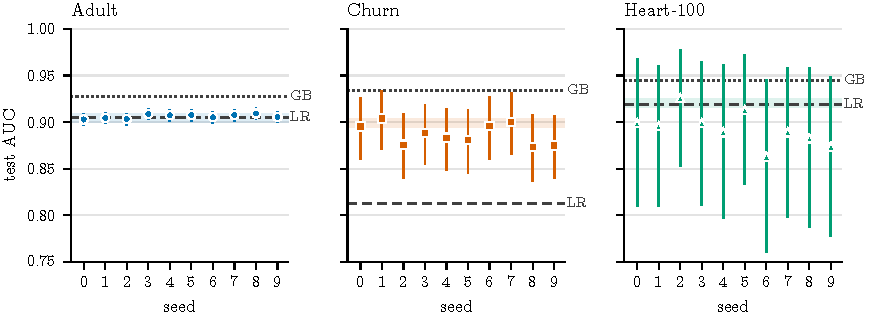
\includegraphics[width=\textwidth,height=0.8\textheight,keepaspectratio]{figures/ch7/used/exp2-auc}
  \caption{Test AUC of each seed's network, with its 95\% interval. Shaded: within 0.01 of the best seed. Dashed: logistic regression (LR); dotted: gradient boosting (GB).}
  \label{fig:exp2-auc}
\end{figure}

% Generated by thesis/ch7/exp2/make_assets.py -- do not edit by hand.
\begin{figure}[tbp]
  \centering
  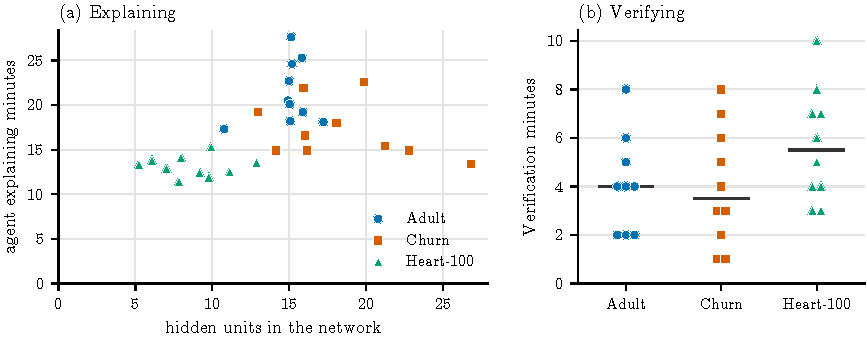
\includegraphics[width=\textwidth,height=0.8\textheight,keepaspectratio]{figures/ch7/options/exp2-cost}
  \caption{Cost of explaining and verifying, one mark per network. (a) The explaining agent's minutes against network size. (b) Verification minutes; bar: median per study.}
  \label{fig:exp2-cost}
\end{figure}

\clearpage
\section*{Heart}
% Generated by thesis/ch7/exp2/make_assets.py -- do not edit by hand.
\begin{table}[tbp]
  \centering
  \footnotesize
  \begin{tabularx}{\textwidth}{@{}>{\raggedright\arraybackslash}X>{\raggedright\arraybackslash}p{3.3cm}ccc@{}}
    \toprule
    Model & Settings & Test AUC & 95\% interval & CV AUC \\
    \midrule
    \multicolumn{5}{@{}l}{\textit{PropNEAT networks}} \\
    The paper's Heart network (40 generations) & -- & 0.897 & [0.808, 0.966] & -- \\
    Heart-100, best seed (s2) & -- & 0.926 & [0.853, 0.978] & -- \\
    Heart-100, median of ten seeds & -- & 0.892 & range 0.863--0.926 & -- \\
    Heart-100, mean prediction of ten seeds & -- & 0.904 & -- & -- \\
    \midrule
    \multicolumn{5}{@{}l}{\textit{Comparators, tuned by 5-fold CV on the training rows}} \\
    Random forest & depth~5, min.\ leaf~5 & 0.949 & [0.887, 0.991] & 0.900 \\
    Explainable boosting machine & interactions~0, bins~32 & 0.947 & [0.886, 0.990] & 0.902 \\
    Gradient boosting, tuned & $L_2$~1, rate~0.03, iterations~100, leaves~7, min.\ leaf~20 & 0.945 & [0.885, 0.988] & 0.888 \\
    Logistic regression ($L_1$, sparse) & $C$~0.3 & 0.926 & [0.849, 0.983] & 0.905 \\
    Logistic regression ($L_2$) & $C$~0.1 & 0.919 & [0.841, 0.978] & 0.905 \\
    Gradient boosting, default settings & -- & 0.918 & -- & -- \\
    MLP, one hidden layer & $\alpha$~1, hidden units~8 & 0.904 & [0.819, 0.969] & 0.888 \\
    Decision tree & depth~6, min.\ leaf~10 & 0.855 & [0.750, 0.944] & 0.823 \\
    \bottomrule
  \end{tabularx}
  \caption{Heart on the paper's split (242 training and 61 test patients). Intervals are 95\% percentile intervals from 10{,}000 bootstrap resamples of the test set (seed 42). CV AUC is the cross-validated AUC on the training rows that chose the settings. The median of ten seeds is not one network, so its range across seeds is given instead of an interval. With 61 test patients the intervals are about 0.1 wide and overlap throughout.}
  \label{tab:exp2-heart-benchmark}
\end{table}

% Generated by thesis/ch7/exp2/make_assets.py -- do not edit by hand.
\begin{table}[tbp]
  \centering
  \small
  \textit{(a) Full against linearised networks}\par\smallskip
  \begin{tabular}{@{}lccc@{}}
    \toprule
    Mean over the ten networks & Full network & Linearised & Gain \\
    \midrule
    Train AUC (242 patients) & 0.956 & 0.927 & $+$0.029 \\
    Test AUC (61 patients) & 0.893 & 0.891 & $+$0.002 \\
    \bottomrule
  \end{tabular}
  \par\bigskip
  \textit{(b) Every non-linear unit and part}\par\smallskip
  \begin{adjustbox}{max width=\textwidth}
  \begin{tabular}{@{}lcccccc@{}}
    \toprule
    & Total & \makecell{Test gain\\CI $>0$} & \makecell{No measurable\\test effect} & Recurring & \makecell{Seed-\\specific} & \makecell{Small support\\($n<30$)} \\
    \midrule
    Non-linear units & 62 & 1 & 61 & 19 & 28 & 16 \\
    Non-linear parts & 45 & 1 & 44 & 9 & 27 & 6 \\
    \bottomrule
  \end{tabular}
  \end{adjustbox}
  \caption{Heart-100 audit: how much of the ten networks' non-linear structure shows on new patients. (a) Each network against itself with every non-linear unit replaced by its best straight line on the training rows; 93\% of the mean training gain does not carry over to the test set, the linearised network does as well or better on test in 5 of 10, and no network has a test-gain interval above zero. (b) A unit or part \emph{generalises} when its own test gain has a 95\% interval above zero; \emph{recurring} means another seed's network reproduces its non-linear residual. Units and parts too close to linear to match (15 and 9) are counted in neither. Binary one-step units are treated as linear. Exploratory, not pre-registered; test numbers were never used to choose.}
  \label{tab:exp2-heart-audit}
\end{table}

% Generated by thesis/ch7/exp2/make_assets.py -- do not edit by hand.
\begin{figure}[tbp]
  \centering
  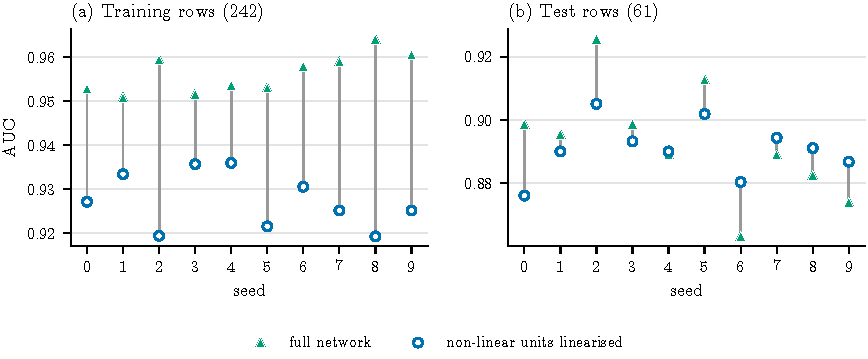
\includegraphics[width=\textwidth,height=0.8\textheight,keepaspectratio]{figures/ch7/exp2-heart-linearised.pdf}
  \caption{Heart-100: each network's AUC with and without its non-linear units.}
  \label{fig:exp2-heart-linearised}
\end{figure}

% Generated by thesis/ch7/exp2/make_assets.py -- do not edit by hand.
\begin{table}[tbp]
  \centering
  \footnotesize
  \begin{tabularx}{\textwidth}{@{}>{\raggedright\arraybackslash}X>{\raggedright\arraybackslash}p{1.5cm}ccccc@{}}
    \toprule
    Family & Seeds & Units & \makecell{Raises /\\lowers risk} & \makecell{Train gain,\\median (max)} & \makecell{Test gain,\\range of estimates} & \makecell{Test CI\\$>0$ / $<0$} \\
    \midrule
    Thallium scan (with ST depression) & s0, s2, s5, s7, s8, s9 & 13 & 10 / 3 & $+$0.0046 ($+$0.0336) & $-$0.001 to $+$0.012 & 0 / 0 \\
    Thallium scan $\times$ age & s2 & 2 & 1 / 1 & $+$0.0057 ($+$0.0093) & $+$0.014 to $+$0.034 & 1 / 0 \\
    Resting blood pressure & s3, s4, s5, s8 & 7 & 4 / 3 & $+$0.0004 ($+$0.0082) & $-$0.005 to $+$0.004 & 0 / 0 \\
    Exercise angina & s0, s4, s6, s9 & 7 & 3 / 4 & $+$0.0072 ($+$0.0163) & $-$0.017 to $+$0.004 & 0 / 0 \\
    Age & s2, s3, s8, s9 & 6 & 1 / 5 & $+$0.0044 ($+$0.0095) & $-$0.006 to $+$0.012 & 0 / 0 \\
    \bottomrule
  \end{tabularx}
  \caption{Heart-100 audit: the non-linear units whose switch is driven by the four inputs of interest, by family. A unit belongs to the family of the inputs that flip it on or off; \emph{raises} or \emph{lowers} is the effect of the unit being on, relative to its straight-line fit. Gains are in AUC when the unit is linearised (train) and on the 61 test patients. The thallium gates recur in idea across seeds but not in mechanism, and none of these families has a measurable test effect, apart from one thallium $\times$ age unit (s2).}
  \label{tab:exp2-heart-families}
\end{table}

% Generated by thesis/ch7/exp2/make_assets.py -- do not edit by hand.
\begin{table}[tbp]
  \thesistablestyle
  \centering
  \footnotesize
  \begin{adjustbox}{max width=\textwidth}
  \begin{tabular}{@{}llcccccc@{}}
    \toprule
    & & \multicolumn{2}{c}{Linear path} & \multicolumn{3}{c}{Average effect, all ten networks} & \\
    \cmidrule(lr){3-4}\cmidrule(lr){5-7}
    Input & Per & \makecell{Networks\\($+$ / $-$)} & Same sign & $+$ / $-$ & Median (min to max) & Spread & LR \\
    \midrule
    Age & year & 9 (8 / 1) & mostly & 10 / 0 & $+$0.024 ($+$0.0019 to $+$0.06) & 31-fold & $+$0.014 \\
    Female (vs male) & level & 9 (0 / 9) & yes & 0 / 10 & $-$2.22 ($-$2.61 to $-$1.34) & 2-fold & $-$1.92 \\
    Typical angina & level & 10 (0 / 10) & yes & 0 / 10 & $-$2.46 ($-$3.76 to $-$0.95) & 4-fold & $-$2.10 \\
    Atypical angina & level & 10 (1 / 9) & mostly & 1 / 9 & $-$0.89 ($-$1.62 to $+$0.0024) & -- & $-$0.80 \\
    Non-anginal pain & level & 10 (0 / 10) & yes & 0 / 10 & $-$1.75 ($-$2.22 to $-$1.30) & 2-fold & $-$1.58 \\
    Resting blood pressure & mm Hg & 5 (5 / 0) & rarely used & 8 / 0 & $+$0.018 (0 to $+$0.041) & 7-fold & $+$0.02 \\
    Cholesterol & mg/dL & 10 (10 / 0) & yes & 10 / 0 & $+$0.013 ($+$0.01 to $+$0.015) & 1-fold & $+$0.0097 \\
    Fasting sugar $>120$ & level & 8 (1 / 7) & mostly & 1 / 7 & $-$0.67 ($-$1.32 to $+$0.077) & -- & $-$0.61 \\
    ECG: ST-T abnormality & level & 5 (4 / 1) & rarely used & 4 / 2 & 0 ($-$0.27 to $+$1.02) & -- & $+$0.42 \\
    ECG: LV hypertrophy & level & 7 (7 / 0) & mostly & 7 / 1 & $+$0.21 ($-$0.0034 to $+$0.36) & -- & $+$0.20 \\
    Maximum heart rate & beat/min & 6 (1 / 5) & mostly & 0 / 10 & $-$0.013 ($-$0.022 to $-$0.004) & 6-fold & $-$0.0077 \\
    Exercise angina & level & 6 (4 / 2) & no & 8 / 0 & $+$0.74 (0 to $+$1.27) & 2-fold & $+$0.62 \\
    ST depression & mm & 3 (3 / 0) & rarely used & 9 / 1 & $+$0.69 ($-$0.12 to $+$0.99) & -- & $+$0.38 \\
    Flat ST slope & level & 10 (10 / 0) & yes & 10 / 0 & $+$1.96 ($+$1.71 to $+$2.32) & 1-fold & $+$1.65 \\
    Downsloping ST slope & level & 9 (5 / 4) & no & 7 / 3 & $+$0.41 ($-$0.59 to $+$1.65) & -- & $+$0.28 \\
    Vessels coloured & vessel & 10 (10 / 0) & yes & 10 / 0 & $+$1.54 ($+$1.25 to $+$1.74) & 1-fold & $+$1.35 \\
    Thallium: not recorded & level & 7 (7 / 0) & mostly & 9 / 0 & $+$2.36 (0 to $+$7.52) & 6-fold & $+$2.26 \\
    Thallium: fixed defect & level & 7 (1 / 6) & mostly & 0 / 9 & $-$0.82 ($-$2.00 to 0) & 8-fold & $-$0.58 \\
    Thallium: reversible defect & level & 8 (7 / 1) & mostly & 10 / 0 & $+$1.38 ($+$1.01 to $+$1.88) & 2-fold & $+$0.96 \\
    \bottomrule
  \end{tabular}
  \end{adjustbox}
  \caption{Heart-100: the linear core across the ten networks, in log-odds per real unit (categories against their reference level). \emph{Linear path}: the coefficient along paths with no switching unit, in the networks that have one; it is shared when every such network gives the same sign (at least 8 networks) or at least 80\% do (at least 6). \emph{Average effect}: the mean change in the score over the training patients, all paths included. Spread is the largest over the smallest non-zero average effect when all agree in sign. LR: logistic regression on the training rows, for reference. Direction is shared; size is not.}
  \label{tab:exp2-linear-core}
\end{table}

% Generated by thesis/ch7/exp2/make_assets.py -- do not edit by hand.
\begin{table}[tbp]
  \thesistablestyle
  \centering
  \footnotesize
  \begin{tabularx}{\textwidth}{@{}cr>{\raggedright\arraybackslash}p{2.3cm}>{\raggedright\arraybackslash}X>{\raggedright\arraybackslash}p{3.3cm}@{}}
    \toprule
    Family & $n$ & Shape & Defining condition (members / patients it covers) & \makecell[l]{Units whose bends\\make the shape} \\
    \midrule
    F1 & 76 & rises $\to$ flat $\to$ rises & age $>$ 65.5 years, thal $\neq$ reversible defect (20/20) & 2116 off (100\%); 855 on (95\%); 2445 on (75\%); 4037 on (51\%) \\
    F2 & 66 & rises & chest pain $\neq$ typical angina, ST slope $\neq$ upsloping, thal = reversible defect (47/53) & 2116 off (100\%); 2445 on (76\%); 4037 on (56\%) \\
    F3 & 50 & rises $\to$ flat $\to$ falls $\to$ rises & age $<$ 63.5 years, age $>$ 45.5 years, ST depression $<$ 0.8 mm (41/77) & 2445 on (100\%); 2116 off (100\%); 4037 on (100\%); 855 on (100\%) \\
    F4 & 36 & rises $\to$ falls $\to$ rises & age $<$ 44.5 years, exercise angina = none (30/33) & 2116 off (100\%); 855 on (100\%); 4037 on (64\%) \\
    F5 & 14 & rises $\to$ flat $\to$ falls & age $<$ 63.5 years, chest pain = typical angina, peak heart rate $<$ 174.5 beat/min (10/11) & 2116 off (100\%); 2445 on (100\%); 4037 on (100\%) \\
    \bottomrule
  \end{tabularx}
  \caption{Heart-100 seed 8: the families of resting-blood-pressure curves. Each of the 242 training patients' predicted risk is traced as resting blood pressure moves over its training range (94 to 200~mm Hg) with everything else held; curves with the same sequence of rises, falls and flat stretches form a family. The defining condition is the decision-tree leaf where the family is the majority. The units are the switches whose bends make the family's shape, with the share of members whose curve has that bend. Unit 2116 is a low-pressure discount and 4037 the fitness readout (part \emph{fitness pathway}), 2445 the fitness score feeding it (\emph{fitness score}) and 855 the ischaemia gate (\emph{ischaemia gate}).}
  \label{tab:exp2-s8-families}
\end{table}

% Generated by thesis/ch7/exp2/make_assets.py -- do not edit by hand.
\begin{figure}[tbp]
  \centering
  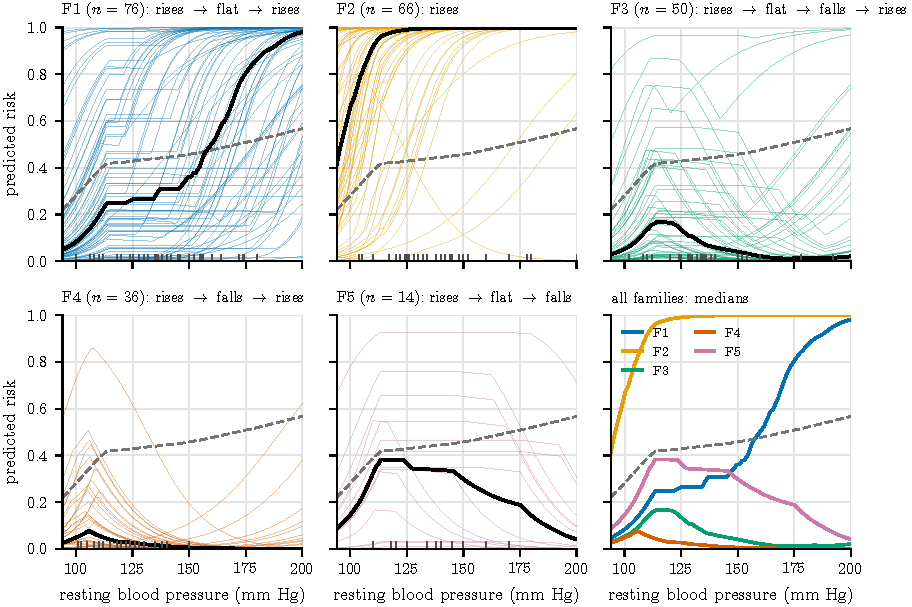
\includegraphics[width=\textwidth,height=0.8\textheight,keepaspectratio]{figures/ch7/used/exp2-s8-ice}
  \caption{Heart-100 seed 8: individual conditional expectation (ICE) curves of predicted risk against resting blood pressure, one panel per shape family. Thin coloured: one training patient; black: the family's median curve; grey dashed: mean of all curves; ticks on the axis: the family's own blood pressures. Last panel: the family medians together.}
  \label{fig:exp2-s8-ice}
\end{figure}

% Generated by thesis/ch7/exp2/make_assets.py -- do not edit by hand.
\begin{figure}[tbp]
  \centering
  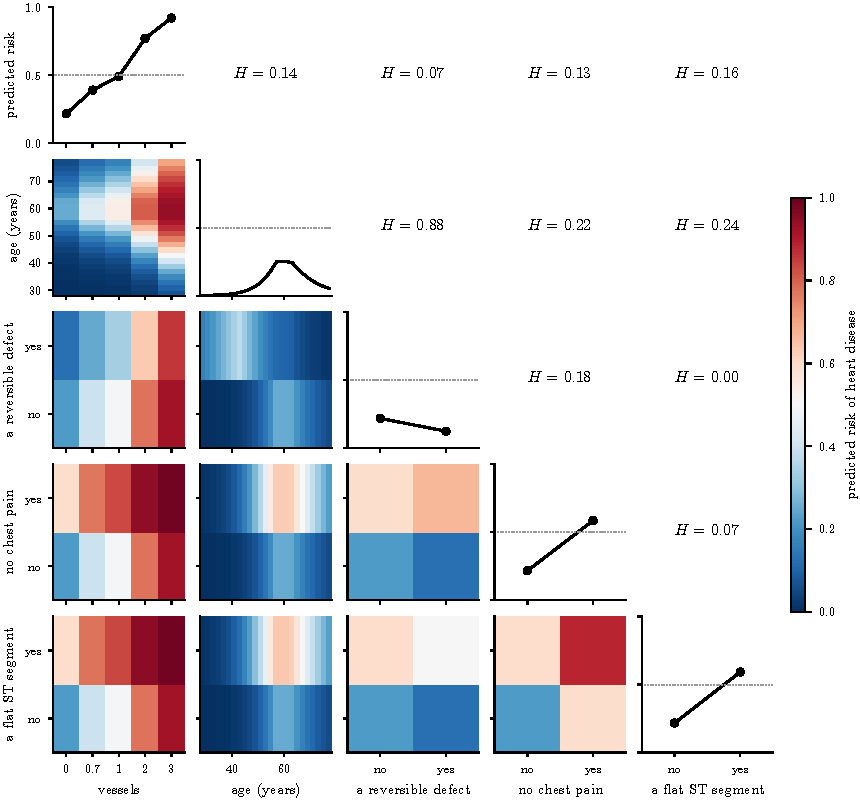
\includegraphics[width=0.95\textwidth,height=0.8\textheight,keepaspectratio]{figures/ch7/exp2-heart-pairs.pdf}
  \caption{Heart-100 seed 2, the whole model: a pairs plot over 5 inputs. Diagonal: predicted risk as one input varies; below the diagonal: as two vary together (colour, centred on a risk of 0.5); above the diagonal: the interaction strength $H$.}
  \label{fig:exp2-heart-pairs}
\end{figure}

\clearpage
\section*{Churn}
% Generated by thesis/ch7/exp2/make_assets.py -- do not edit by hand.
\begin{table}[tbp]
  \thesistablestyle
  \centering
  \footnotesize
  \begin{tabularx}{\textwidth}{@{}>{\raggedright\arraybackslash}Xcccc@{}}
    \toprule
    Signal & \makecell{Relevance\\(CV)} & \makecell{Seeds\\using} & \makecell{Gain, median\\train / test} & \makecell{Seeds with test\\CI $>0$ ($<0$)} \\
    \midrule
    \multicolumn{5}{@{}l}{\textit{Core: used by every seed}} \\
    \quad International plan, offset & $+$0.040 & 10 & 0.064 / 0.075 & 10 \\
    \quad Service calls, slope & $+$0.027 & 10 & 0.025 / 0.034 & 10 \\
    \quad Service-call threshold & $+$0.022 & 10 & 0.010 / 0.009 & 3 \\
    \quad Heavy-day hinge & $+$0.017 & 10 & 0.014 / 0.018 & 7 \\
    \quad Day usage, slope & $+$0.015 & 10 & 0.010 / 0.007 & 3 \\
    \quad Evening usage, slope & $+$0.012 & 10 & 0.003 / 0.009 & 8 \\
    \quad Voice mail, offset & $+$0.010 & 10 & 0.005 / 0.006 & 2 \\
    \quad State offsets$^\dagger$ & $-$0.001 & 10 & 0.009 / $-$0.005 & 0 (1) \\
    \quad Night usage, slope & $-$0.003 & 10 & 0.001 / 0.004 & 5 \\
    \midrule
    \multicolumn{5}{@{}l}{\textit{Common: used by 4 to 9 seeds}} \\
    \quad Day $+$ evening bill & $+$0.024 & 9 & 0.008 / 0.007 & 3 \\
    \quad International minutes, slope & $+$0.010 & 9 & 0.002 / 0.002 & 0 \\
    \quad Service calls $\times$ light day use & $+$0.021 & 8 & 0.009 / 0.012 & 8 \\
    \quad Evening bend$^\dagger$ & $-$0.006 & 7 & $-$0.001 / 0.002 & 0 \\
    \quad Day calls, slope$^\dagger$ & $+$0.002 & 6 & 0.001 / $-$0.003 & 0 (3) \\
    \quad Account length, slope & $+$0.001 & 5 & 0.001 / $-$0.001 & 0 \\
    \quad Heavy day use without voice mail & $+$0.020 & 4 & 0.006 / 0.006 & 3 \\
    \quad International calls, slope & $+$0.001 & 4 & 0.001 / 0.001 & 0 \\
    \midrule
    \multicolumn{5}{@{}l}{\textit{Rare: used by 1 to 2 seeds}} \\
    \quad Service calls $\times$ voice mail$^\dagger$ & $-$0.000 & 2 & $-$0.000 / 0.001 & 0 \\
    \quad International-minutes bend & $+$0.008 & 1 & 0.000 / 0.000 & 0 \\
    \quad Day $\times$ night usage & $+$0.008 & 1 & 0.001 / $-$0.001 & 0 \\
    \quad Evening usage $\times$ service calls$^\dagger$ & $-$0.003 & 1 & 0.001 / 0.000 & 0 \\
    \midrule
    \multicolumn{5}{@{}l}{\textit{Absent from every network (relevant in the data)}} \\
    \quad International plan $\times$ international use & $+$0.047 & 0 & \multicolumn{2}{c}{data's own: test 0.015 [0.003, 0.026]} \\
    \quad International-calls bend & $+$0.003 & 0 & \multicolumn{2}{c}{data's own: test 0.004 [$-$0.003, 0.013]} \\
    \bottomrule
  \end{tabularx}
  \caption{Churn: the signals of the ten networks. A signal is a churn-relevant function of the inputs, defined on the data and independent of any model. \emph{Relevance}: the cross-validated log-loss gain when the signal is added to a ridge logistic fit on the training rows. A seed \emph{uses} a signal when its own component has a standard deviation of at least 0.10 logit (training rows, after clipping to its 1st--99th percentiles). \emph{Gain}: AUC lost when that component is removed (median over the seeds using it). $^\dagger$Noise: the data do not support it or it never helps on test. The strongest interaction in the data, international plan $\times$ international use, is in no network.}
  \label{tab:exp2-churn-signals}
\end{table}

% Generated by thesis/ch7/exp2/make_assets.py -- do not edit by hand.
\begin{table}[tbp]
  \thesistablestyle
  \centering
  \footnotesize
  \begin{adjustbox}{max width=\textwidth}
  \setlength{\tabcolsep}{3pt}
  \begin{tabular}{@{}lcccccccccccc@{}}
    \toprule
    Seed & \rotatebox{70}{Calls slope} & \rotatebox{70}{Calls threshold} & \rotatebox{70}{Calls $\times$ light day} & \rotatebox{70}{Day slope} & \rotatebox{70}{Day hinge} & \rotatebox{70}{Day $+$ eve bill} & \rotatebox{70}{Day w/o voice mail} & \rotatebox{70}{Evening} & \rotatebox{70}{Intl plan} & \rotatebox{70}{Voice mail} & \rotatebox{70}{State} & \rotatebox{70}{Plan $\times$ intl use} \\
    \midrule
    s0 & 0.73 & \makecell{0.53\\{\scriptsize S4/3p}} & \makecell{0.33\\{\scriptsize S3/2p}} & 0.53 & \makecell{0.86\\{\scriptsize S4/3p}} & \makecell{0.40\\{\scriptsize S2/1p}} & \makecell{0.24\\{\scriptsize H/1p}} & 0.32 & 0.82 & 0.50 & 0.51 & -- \\
    s1 & 0.72 & \makecell{0.57\\{\scriptsize S2/1p}} & \makecell{0.33\\{\scriptsize H/1p}} & 0.66 & \makecell{0.99\\{\scriptsize S4/2p}} & \makecell{0.40\\{\scriptsize S2/1p}} & \makecell{0.38\\{\scriptsize H/1p}} & 0.45 & 0.85 & 0.45 & 0.51 & -- \\
    s2 & 0.85 & \makecell{0.60\\{\scriptsize S8/4p}} & \makecell{0.41\\{\scriptsize S6/3p}} & 0.56 & \makecell{0.80\\{\scriptsize S4/2p}} & \makecell{0.38\\{\scriptsize S4/2p}} & -- & 0.37 & 0.79 & 0.74 & 0.60 & -- \\
    s3 & 0.74 & \makecell{0.40\\{\scriptsize G/1p}} & \makecell{0.29\\{\scriptsize S3/2p}} & 0.68 & \makecell{0.74\\{\scriptsize S3/1p}} & \makecell{0.40\\{\scriptsize S2/1p}} & -- & 0.29 & 0.78 & 0.55 & 0.53 & -- \\
    s4 & 0.69 & \makecell{0.43\\{\scriptsize G/1p}} & w & 0.87 & \makecell{0.64\\{\scriptsize G/1p}} & \makecell{0.44\\{\scriptsize S2/1p}} & -- & 0.38 & 0.77 & 0.58 & 0.63 & -- \\
    s5 & 0.81 & \makecell{0.56\\{\scriptsize S4/1p}} & \makecell{\textbf{0.69}\\{\scriptsize S5/1p}} & 0.68 & \makecell{0.71\\{\scriptsize S4/2p}} & -- & -- & 0.48 & 0.78 & 0.60 & 0.47 & -- \\
    s6 & 0.88 & \makecell{0.50\\{\scriptsize S4/1p}} & \makecell{0.47\\{\scriptsize S5/2p}} & 0.55 & \makecell{0.86\\{\scriptsize S2/2p}} & \makecell{0.39\\{\scriptsize G/1p}} & \makecell{0.49\\{\scriptsize G/1p}} & 0.33 & 0.92 & 0.52 & 0.69 & -- \\
    s7 & 0.74 & \makecell{0.52\\{\scriptsize S2/2p}} & \makecell{0.25\\{\scriptsize S3/2p}} & 0.84 & \makecell{0.84\\{\scriptsize S5/3p}} & \makecell{0.50\\{\scriptsize S5/3p}} & \makecell{0.63\\{\scriptsize S5/3p}} & 0.25 & 0.88 & 0.41 & 0.55 & -- \\
    s8 & 0.68 & \makecell{0.53\\{\scriptsize S4/2p}} & \makecell{0.37\\{\scriptsize S4/2p}} & 0.51 & \makecell{0.64\\{\scriptsize S2/2p}} & \makecell{0.27\\{\scriptsize G/1p}} & -- & 0.32 & 0.70 & 0.57 & 0.59 & -- \\
    s9 & 0.61 & \makecell{0.48\\{\scriptsize H/1p}} & -- & 0.67 & \makecell{0.58\\{\scriptsize S5/2p}} & \makecell{0.30\\{\scriptsize S4/1p}} & -- & 0.29 & 0.76 & 0.47 & 0.54 & -- \\
    \bottomrule
  \end{tabular}
  \end{adjustbox}
  \caption{Churn: how each seed realises the main signals. Each cell is the standard deviation of the network's own component for that signal (logit, training rows). For a non-linear signal the second line gives its realisation: H, a single hinge on one input; G, a single gate (one unit that also reads another input); S$k$, split across $k$ units; /$n$p, spread over $n$ explanation parts. w: weak (0.03 to 0.10 logit); --: not used. Bold: the strongest calls $\times$ light-day realisation (s5). Every seed has the same core signals, assembled differently; no seed has the international plan $\times$ international use interaction.}
  \label{tab:exp2-churn-matrix}
\end{table}

% Generated by thesis/ch7/exp2/make_assets.py -- do not edit by hand.
\begin{figure}[tbp]
  \centering
  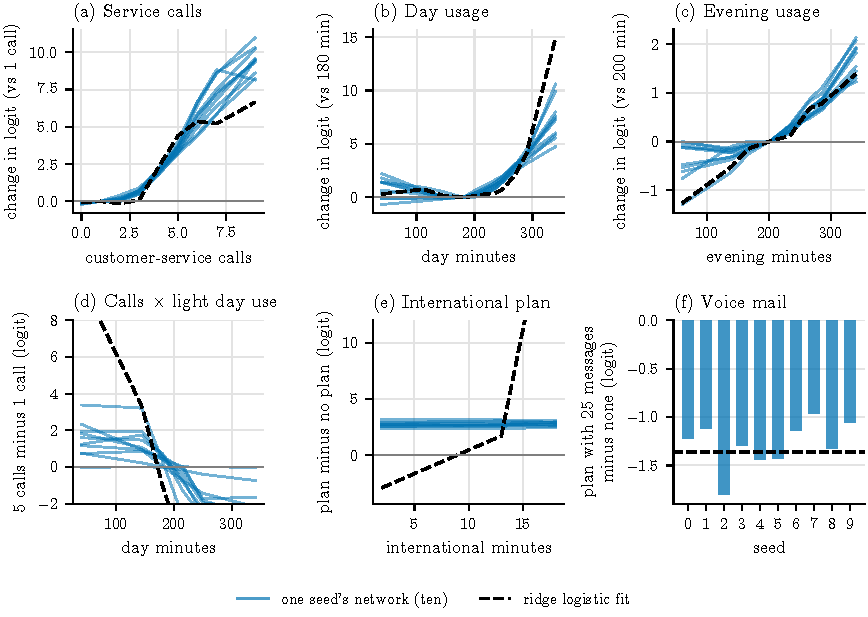
\includegraphics[width=\textwidth,height=0.8\textheight,keepaspectratio]{figures/ch7/exp2-churn-shapes.pdf}
  \caption{Churn: each signal's shape in the ten networks, as a change in the churn score (logit). Blue: one seed's network (one line or bar per seed); dashed: ridge logistic fit.}
  \label{fig:exp2-churn-shapes}
\end{figure}

% Generated by thesis/ch7/exp2/make_assets.py -- do not edit by hand.
\begin{figure}[tbp]
  \centering
  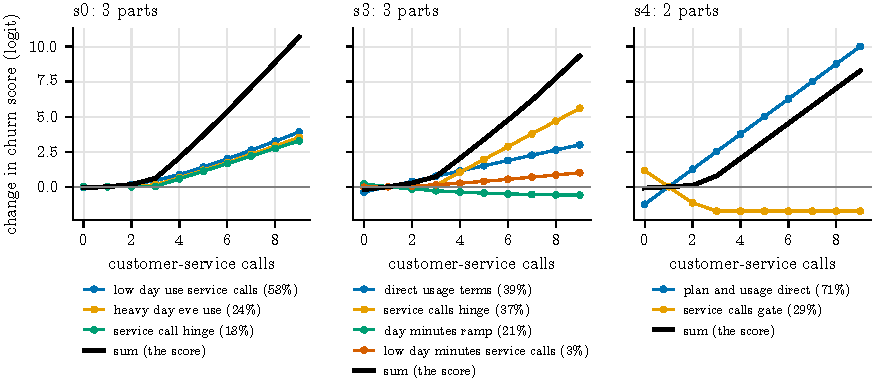
\includegraphics[width=\textwidth,height=0.8\textheight,keepaspectratio]{figures/ch7/used/exp2-churn-calls-parts}
  \caption{Churn: one signal, three realisations. The score's response to customer-service calls (relative to 1 call), split into the explanation parts that carry it; black: their sum, the score's response. Legend: each part's share of the response's variance.}
  \label{fig:exp2-churn-calls-parts}
\end{figure}

% Generated by thesis/ch7/exp2/make_assets.py -- do not edit by hand.
\begin{figure}[tbp]
  \centering
  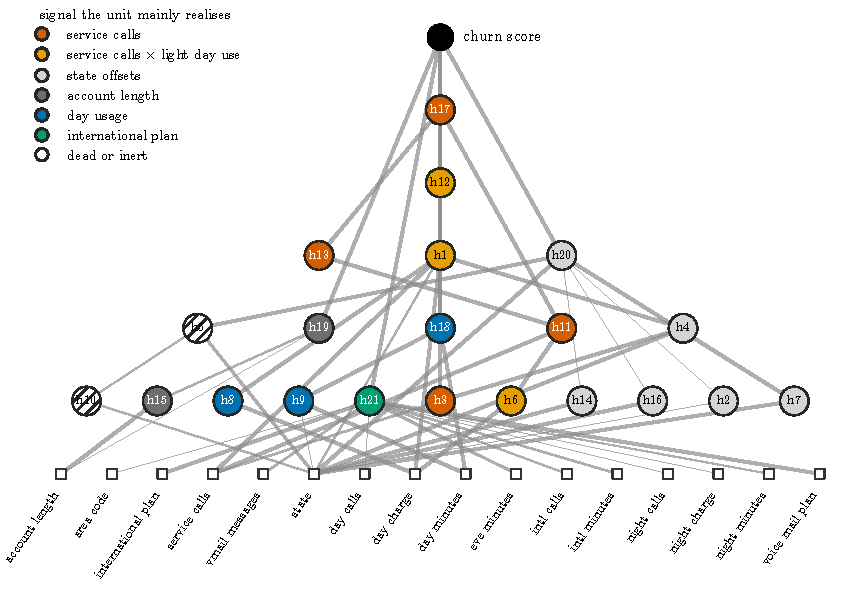
\includegraphics[width=\textwidth,height=0.8\textheight,keepaspectratio]{figures/ch7/exp2-churn-s5-network.pdf}
  \caption{Churn seed 5: every hidden node, coloured by the signal it mainly realises. The 31 state indicators are drawn as one input; line width: absolute weight.}
  \label{fig:exp2-churn-s5-network}
\end{figure}

% Generated by thesis/ch7/exp2/make_assets.py -- do not edit by hand.
\begin{table}[tbp]
  \centering
  \small
  \begin{tabularx}{\textwidth}{@{}Xccc@{}}
    \toprule
    & \makecell{Share of\\disagreement} & \multicolumn{2}{c}{\makecell{Agreement after replacing it\\by the ten-seed average}} \\
    \cmidrule(l){3-4}
    Source of disagreement & & \makecell{Median logit\\correlation} & \makecell{Median top-141\\overlap} \\
    \midrule
    As trained & -- & 0.890 & 79\% \\
    \midrule
    State offsets & 22\% & 0.912 & 83\% \\
    Heavy-usage complex: day slope and hinge, day $+$ evening bill, day without voice mail, evening & 38\% & 0.935 & 83\% \\
    Service-call complex: slope and threshold, calls $\times$ light day use & 15\% & 0.906 & 84\% \\
    Night and international usage & 6\% & 0.897 & 82\% \\
    Other signals: voice mail, international plan, account and call counts, minor interactions & 8\% & -- & -- \\
    Residual: not in the signal list (three-way and state $\times$ usage gates) & 11\% & -- & -- \\
    \midrule
    Every signal except the state offsets & -- & 0.962 & 90\% \\
    Every signal (only the residual differs) & -- & 0.990 & 94\% \\
    State inputs held at their training average & -- & 0.909 & 80\% \\
    \bottomrule
  \end{tabularx}
  \caption{Churn: where the ten networks disagree, on the 1{,}000 test customers. Each pair's difference in logit is split into the signals' contributions; a signal's share is the covariance of its difference with the total difference over the variance of the total (mean over the 45 pairs; the shares sum to one). The right-hand columns replace that signal's realisation in every network by the ten-seed average and measure agreement again; the top-141 overlap compares each pair's 141 riskiest customers (the number who churned). Holding the state inputs at their average also raises the median test AUC from 0.886 to 0.894.}
  \label{tab:exp2-churn-disagreement}
\end{table}

% Generated by thesis/ch7/exp2/make_assets.py -- do not edit by hand.
\begin{table}[tbp]
  \centering
  \small
  \begin{tabular}{@{}lc@{}}
    \toprule
    \multicolumn{2}{@{}l}{\textit{Churn on the training rows}} \\
    International plan, at most 2 international calls & 69 of 69 (100\%) \\
    International plan, more than 13 international minutes & 66 of 66 (100\%) \\
    International plan, neither & 33 of 252 (13\%) \\
    No international plan & 405 of 3{,}620 (11\%) \\
    \midrule
    \multicolumn{2}{@{}l}{\textit{Test AUC}} \\
    Ridge logistic fit on the signal list, with this interaction & 0.922 \\
    The ten networks & 0.873--0.904 \\
    Their mean prediction & 0.899 \\
    \bottomrule
  \end{tabular}
  \caption{Churn: the signal no network has. Customers with an international plan churn almost surely when they make few international calls or many international minutes; every network treats the plan as a flat offset instead. This interaction is the most relevant signal in the data (cross-validated log-loss gain $+$0.047), and removing it from the ridge fit costs 0.015 test AUC [0.003, 0.026]. No network was trained with it, so its value to a network is untested.}
  \label{tab:exp2-churn-blindspot}
\end{table}

% Generated by thesis/ch7/exp2/make_assets.py -- do not edit by hand.
\begin{table}[tbp]
  \thesistablestyle
  \centering
  \small
  \begin{tabularx}{\textwidth}{@{}>{\raggedright\arraybackslash}Xccc@{}}
    \toprule
    & Churn & \makecell{Churn, state inputs\\at their average} & Heart-100 \\
    \midrule
    Test rows & 1{,}000 & 1{,}000 & 61 \\
    Logit correlation between seeds, median (min) & 0.890 (0.779) & 0.909 (0.792) & 0.921 (0.867) \\
    Rank correlation between seeds, median & 0.860 & 0.879 & 0.934 \\
    Overlap of the top-$k$ riskiest, median (min)$^\dagger$ & 79\% (69\%) & 80\% (71\%) & 91\% (84\%) \\
    Mean absolute difference in predicted risk, median & 0.051 & 0.049 & 0.087 \\
    Test AUC of one seed, median (range) & \makecell{0.886\\(0.873--0.904)} & \makecell{0.894\\(0.882--0.907)} & \makecell{0.892\\(0.863--0.926)} \\
    Test AUC of the ten seeds' mean prediction & 0.899 & 0.904 & 0.904 \\
    \bottomrule
  \end{tabularx}
  \caption{Prediction agreement between the ten seeds on the test rows (45 pairs per study). $^\dagger$The top $k$ is the number of positive test cases: $k=141$ for Churn and $k=32$ for Heart-100. Heart-100's seeds agree more closely with one another than Churn's do; on Churn, holding the state inputs at their training average removes part of the disagreement and slightly raises accuracy.}
  \label{tab:exp2-agreement}
\end{table}

\clearpage
\section*{Worked verification example (churn100-s5, service calls)}
% Generated by thesis/ch7/exp2/make_assets.py -- do not edit by hand.
\begin{table}[tbp]
  \centering
  \footnotesize
  \begin{tabularx}{\textwidth}{@{}>{\raggedright\arraybackslash}X>{\centering\arraybackslash}p{2.3cm}>{\centering\arraybackslash}p{2.3cm}>{\centering\arraybackslash}p{1.6cm}@{}}
    \toprule
    Statement in the hypothesis (query it cites) & \makecell{Stated\\(record)} & \makecell{Recomputed\\(train)} & \makecell{Test\\split} \\
    \midrule
    Probe, typical customer at 120 daytime minutes (day charge \$20.40): predicted risk at 0, 3, 4 calls & 1\% / 16\% / 70\% & 1\% / 16\% / 70\% & -- \\
    Probe, typical customer at 180 daytime minutes (day charge \$30.60): predicted risk at 2, 4, 5 calls & 3\% / 13\% / 57\% & 3\% / 13\% / 57\% & -- \\
    Probe, typical customer at 240 daytime minutes (day charge \$40.80): predicted risk at 0, 6, 7 calls & 15\% / 15\% / 38\% & 15\% / 15\% / 38\% & -- \\
    Customers with calls $\ge$ 4, day charge $<$ \$30: $n$, churn rate, mean predicted risk, part's mean contribution & 156 / 75.6\% / 65.5\% / 5.30 & 156 / 75.6\% / 65.5\% / 5.30 & 38 / 76.3\% / 5.42 \\
    Customers with calls $\ge$ 4, day charge $\ge$ \$30: $n$, churn rate, part's mean contribution & 162 / 25.3\% / 0.20 & 162 / 25.3\% / 0.20 & 43 / 30.2\% / 0.21 \\
    Part switched off (output at its baseline): AUC with / without & 0.901 / 0.759 & 0.901 / 0.759 & 0.881 / 0.738 \\
    Florida-specific unit open (training rows) & 3 & 3 & -- \\
    Rounding error of the three-significant-figure formula (max over training rows) & 0.016 & not rerun & -- \\
    \midrule
    \multicolumn{4}{@{}l}{\textit{Checks on the part and the explanation}} \\
    Part's extracted formula reproduces its output (max abs.\ error, train) & \multicolumn{3}{c}{3.6e-15} \\
    Whole explanation reproduces the network (max abs.\ error) & \multicolumn{3}{c}{4.4e-16} \\
    Interaction claim: effect of calls (0 to 9) with total daytime charge above 30.69 US dollars minus with total daytime charge at or below 30.69 US dollars (log-odds) & \multicolumn{2}{c}{$-$1.67} & agrees \\
    Plain-language claims about the part: verified / test split agrees & \multicolumn{3}{c}{12 of 13 / 6 of 10} \\
    Recheck of the whole record: mismatches / needs review & \multicolumn{3}{c}{0 / 1} \\
    Self-probe of this part by the agent & \multicolumn{3}{c}{done, none refuted} \\
    Verification of the whole network (minutes) & \multicolumn{3}{c}{4} \\
    \bottomrule
  \end{tabularx}
  \caption{Churn seed 5, the part \emph{Service calls and daytime charge}: what was claimed and how it was checked. The agent's hypothesis opens: ``Customer-service calls raise the predicted churn risk steeply once a customer has made several of them while daytime use is low or average; for heavy daytime users the calls make little difference until the count is high.'' Every number in the hypothesis is a reference to a stored query; \emph{Stated} is the value stored with that query when the agent wrote the hypothesis, \emph{Recomputed} the same query run again on the network for this table (19 of 19 values agree as printed), \emph{Test} the same query on the test split (subgroups: $n$ / churn rate / part's mean contribution). The part's mean contribution is in log-odds, relative to the part's training baseline. The rounding-error query (the whole-explanation check) is not rerun here. Interaction claim: the plain-language layer's difference-in-differences of the calls effect between the two day-charge groups; its test verdict compares the same groups on the test split.}
  \label{tab:exp2-worked-claims}
\end{table}

% Generated by thesis/ch7/exp2/worked.py -- do not edit by hand.
\begin{figure}[tbp]
  \centering
  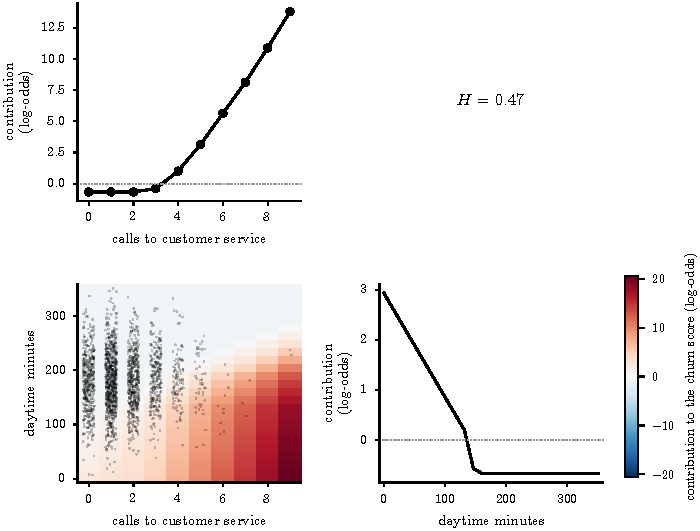
\includegraphics[width=0.85\textwidth,height=0.8\textheight,keepaspectratio]{figures/ch7/used/exp2-worked-pairs}
  \caption{Churn seed 5, the part \emph{Service calls and daytime charge}: a pairs plot of the part's contribution to the churn score (log-odds) over its two main inputs. Diagonal: one input varies; lower left: both together (colour: blue lowers and red raises the score; dots: training customers, calls jittered); upper right: the interaction strength $H$. The daytime charge is drawn in minutes.}
  \label{fig:exp2-worked-pairs}
\end{figure}

% Generated by thesis/ch7/exp2/worked.py -- do not edit by hand.
\begin{figure}[tbp]
  \centering
  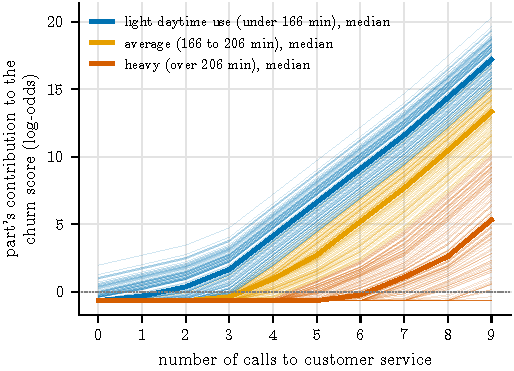
\includegraphics[width=0.7\textwidth,height=0.8\textheight,keepaspectratio]{figures/ch7/exp2-worked-ice.pdf}
  \caption{Churn seed 5, the part \emph{Service calls and daytime charge}: individual conditional expectation (ICE) curves of the part's contribution to the churn score as the number of customer-service calls varies, coloured by the customer's daytime minutes (thirds), with the median curve of each third. 0: the part adds nothing beyond its average.}
  \label{fig:exp2-worked-ice}
\end{figure}

% Generated by thesis/ch7/exp2/worked.py -- do not edit by hand.
\begin{figure}[tbp]
  \centering
  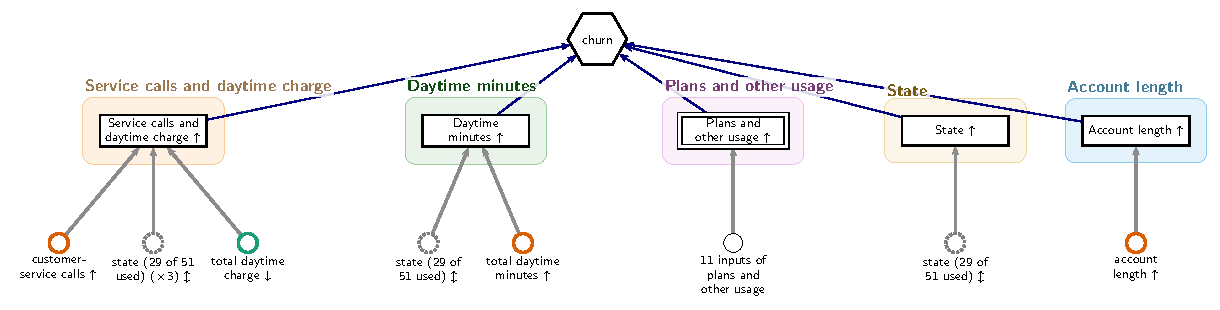
\includegraphics[width=\textwidth,height=0.8\textheight,keepaspectratio]{figures/ch7/used/exp2-worked-net-concept}
  \caption{Churn seed 5 at the level of concepts: each top-level part of the explanation collapsed into one box, the inputs each reads, and the churn score at the top. Arrows on inputs and boxes: the direction of the effect on the final prediction (up raises it, down lowers it, double arrow depends). Edges: blue, a positive weight (raises the score); red, a negative weight; thicker, a larger weight; grey, the inputs a collapsed part reads (no single weight). A grouped input (state) stands for its used levels.}
  \label{fig:exp2-worked-net-concept}
\end{figure}

% Generated by thesis/ch7/exp2/worked.py -- do not edit by hand.
\begin{figure}[tbp]
  \centering
  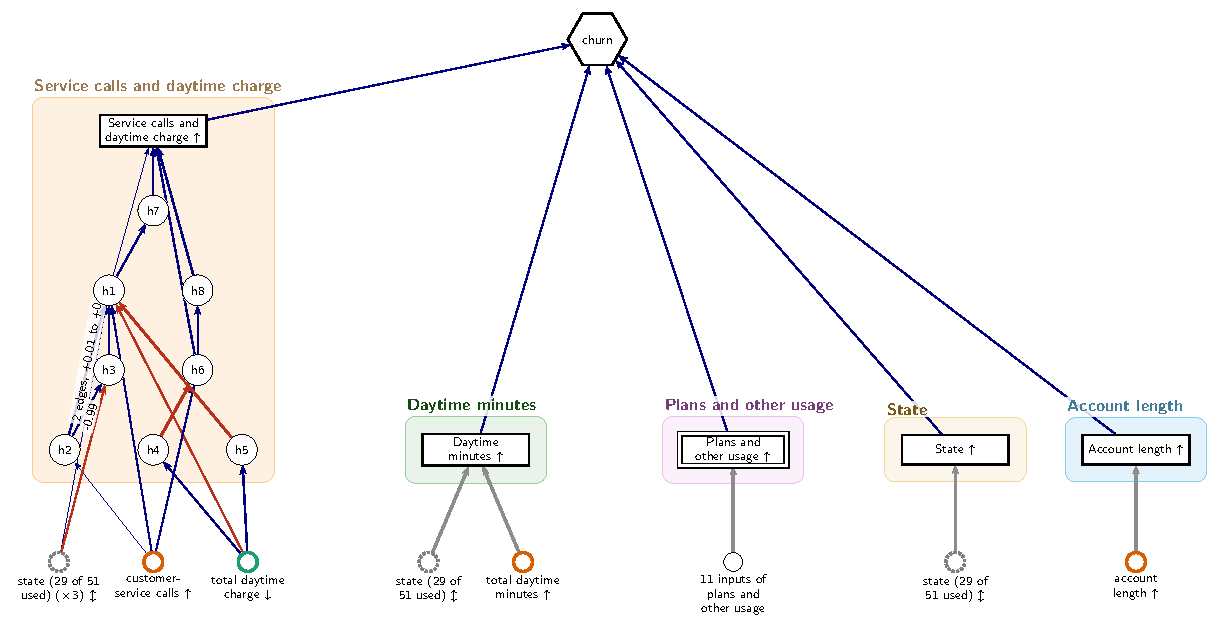
\includegraphics[width=\textwidth,height=0.8\textheight,keepaspectratio]{figures/ch7/used/exp2-worked-net-exploded}
  \caption{Churn seed 5 with the part \emph{Service calls and daytime charge} expanded and the other parts collapsed. Edges: blue, a positive weight (raises the score); red, a negative weight; thicker, a larger weight; grey, the inputs a collapsed part reads (no single weight).}
  \label{fig:exp2-worked-net-exploded}
\end{figure}

% Generated by thesis/ch7/exp2/worked.py -- do not edit by hand.
\begin{figure}[tbp]
  \centering
  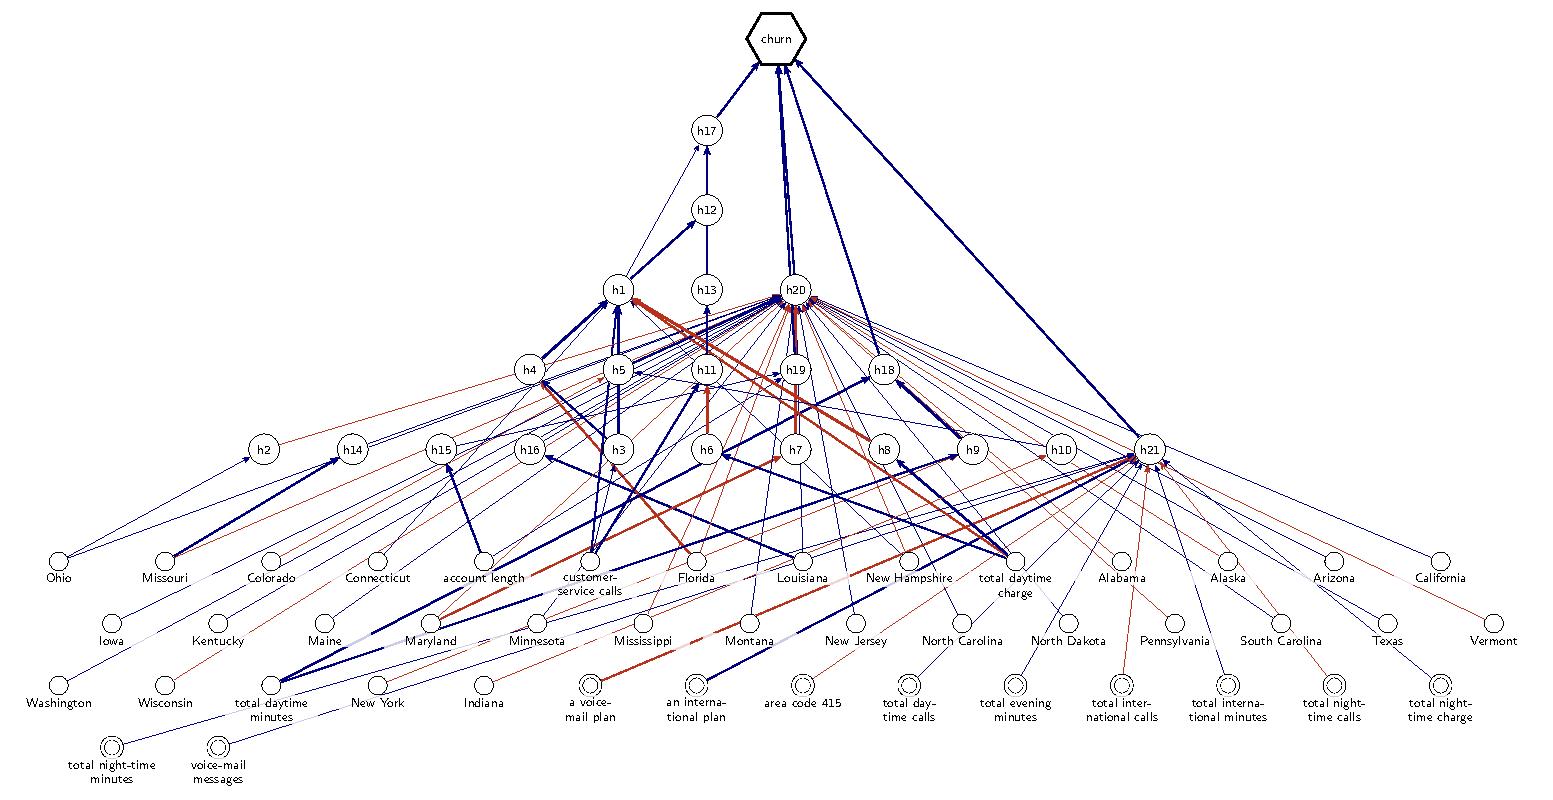
\includegraphics[width=\textwidth,height=0.8\textheight,keepaspectratio]{figures/ch7/exp2-worked-net-unexplained.pdf}
  \caption{Churn seed 5 as trained, before any explanation: input columns (bottom), hidden units (circles) and the output (hexagon). Edges: blue, a positive weight (raises the score); red, a negative weight; thicker, a larger weight. Double outline: an input that acts at a fixed rate.}
  \label{fig:exp2-worked-net-unexplained}
\end{figure}

\end{document}
